%!TEX root = ./thesis.tex

\chapter{Einführung}\label{chapter:intro}

Zweibeiniges Gehen bietet als Fortbewegungsart durch virtuelle Umgebungen viele Vorteile gegenüber alternativen Fortbewegungsarten. Usoh et al \cite{usoh-vergleich-1999} beschreiben beispielsweise, ein höheres Präsenzgefühl der Nutzer:innen, wenn diese sich gehend durch die virtuelle Umgebung fortbewegten, als wenn diese per Knopfdruck durch die Szene flogen.
Eine der drei von LaViola \cite{cybersickness} zusammenfassten Theorien, die \textquote{Sensory Conflict Theory} (Sensorische Konflikt Theorie) erklärt die Ursache für so genannte \textquote{Cybersickness} oder auch Simulatorkrankheit, also dass Nutzer:innen in bestimmten, durch virtuelle Umgebungen hervorgerufenen Situationen teilweise starke Übelkeit erleben so, dass Informationen verschiedener Sinnesmodalitäten widersprüchlich sind.
Demnach wäre es also Cybersickness senkend, wenn andere Sinnesmodalitäten, wie der Gleichgewichtssinn oder die Propriozeption zusätzlich zum visuellen Sinn die Eigenbewegung der Nutzer:in wahrnehmen. Und tatsächlich konnten Langbehn et al \cite{langbehn-vergleich-2018} zeigen, dass Nutzer:innen, die sich in virtuellen Umgebungen fortbewegen signifikant weniger Cybersickness erleben, als wenn sie sich mithilfe von Joysticks fortbewegen.

% erklärt, dass beim Gehen mehr Sinne stimuliert werden als bei künstlichen Alternativen, wie zum Beispiel der Joystick Steuerung. Tiefensensibilität (Propriozeption) und Gleichgewichtssinn (vestibuläre Wahrnehmung) signalisieren, dass er gerade wirklich geht, während diese Information bei alternativen Fortbewegungsart allein vom visuellen Sinn übermittelt wird.
Leider bringt das natürliche gehen (Real-Walking) auch den großen Nachteil mit sich, dass es in der Regel auf einen einzelnen Raum (den Trackingspace) beschränkt ist.

Dies entsteht zum einen, durch räumlich limitierte Erfassung (auf Englisch: tracking) der Position und Rotation von Headset und Controllern bei einigen Technologien, zum anderen durch die Raumgröße der meisten VR-Setups.

Zwar gibt es dazu auch Ausnahmen, ( siehe z.B. \cite{microsoft}
), jedoch sind diese dann mit großem Aufwand verbunden und nicht für jede Endnutzer:in umzusetzen.

\section{Redirection Methoden}
Eine Herangehensweise an dieses Problem sind so genannte \textquote{Redirection Techniques} (besser bekannt als Redirected Walking, diese Begriffe werden oft austauschbar verwendet, siehe \cite{redwalk_uebersicht})). Dies ist ein Sammelbegriff für Methoden bei denen die Nutzer:in durch subtile Manipulationen an der Darstellung der virtuellen Umgebung, auf virtuelle Gebiete zugreifen kann, die sonst außerhalb des begehbaren Bereichs wären. Tatsächlich bleibt sie dabei aber nur innerhalb des realen Trackingspaces.
Im Idealfall wird dabei die Illusion aufrecht erhalten sie würde sich unmanipuliert, frei, und in virtueller und echter Umgebung identisch bewegen. Tatsächlich werden bei den meisten dieser Methoden %unterschied zwischen methode und methodik?
an gewisse Veränderungen zwischen der Nutzer:in und ihrem virtuellen Avatar etabliert (beispielsweise die Geh-Geschwindigkeit), sodass die Bewegung sich zwischen den beiden Umgebungen unterscheiden.
Bei manchen dieser Methoden sorgt diese Veränderung dafür, die Bewegungen der Nutzer:in in gewisser Weise zu Manipulieren, beispielsweise indem diese unbewusst die veränderungen Auszugleichen.

Mit diesen Methoden lassen sich also einige Effekte erzielen, wie unter anderem die virtuell begehbare Fläche zu vergrößern.
Im folgenden werde ich nun zwei dieser Methoden genauer vorstellen.
%%%%%%%%%%%%

\subsection{Rotationgains}
Rotationgains werden Kopfrotationen hinzugefügt sodass sich die virtuelle Kamera leicht schneller oder langsamer dreht als der reale
Kopf mit dem VR-Headset.

Kopfrotationen lassen sich mit der Schreibweise
$$ R_{real} := (pitch_{real}, yaw_{real}, roll_{real}) $$
darstellen (siehe Steinicke et al \cite{detection-thresholds}) %genug zitiert? dieser ganze abschnitt kommt daher
, wobei $pitch$, $yaw$ und $roll$ die Eulerschen Winkel der Kopfrotation darstellen. Ein Rotationgain wird als Quotient des virtuellen Winkels und des realen Winkels einer Rotationsdimension definiert also:
$$ gR := \frac{R_{virtual}}{R_{real}} $$
Für alle 3 Winkel kann ein Rotationgain angewandt werden.
Dieses Anwenden funktioniert indem statt der eigentlichen Rotatation $\alpha$, die Multiplikation aus $\alpha$ mit dem Rotationgain also:
$$ gR * \alpha $$
durchgeführt wird. \cite{detection-thresholds}

Folglich rotieren virtuelle Kameras mit einem Rotationgain von $gR > 1$ schneller in die Richtung der realen Kopfdrehung als der reale Kopf, während solche mit einem Rotationgain von $gR < 1$ langsamer die Richtung drehen.
%nochmal peck 11 angucken dazu
Da für jeden Winkel der Kopfrotation ein Rotationgain definiert werden kann können Rotationgains folgendermaßen dargestellt werden:
$$(gR_{pitch}, gR_{yaw}, gR_{roll})$$
Nach Steinicke et al \cite{detection-thresholds} wird in der Regel für Redirection ein Rotationgain auf den $yaw_{real}$ Winkel der Kopfrotation angewandt.
Durch Anwenden eines positiven Rotationgains auf $yaw$-Rotationen nach rechts und eines neutralen oder sogar negativen, für Rotationen nach Links kann der virtuelle Trackingspace um den realen Trackingspace nach rechts, mit dem Drehpunkt der Nutzerposition herum rotiert werden. Andersherum natürlich genauso. Indem im vorhinein ein Winkel $\beta$, für die Ziel-Verdrehung der beiden Realitäten definiert wird, lässt sich beim Erreichen dieses Winkels das Anwenden des Rotationgains beenden, sodass die Welten sich nun um genau $\beta$ Grad verdreht haben.

Dies ermöglicht Prozesse, bei denen in bestimmten Bereichen der virtuellen Realität ein solcher gerichteter Rotationgain bis zu einem bestimmten Ziel-Winkel um einen vorher definierten Drehpunkt\footnote{Es sollte dafür gesorgt werden, dass dieser möglichst nah an der Position des virtuellen Avatar liegt, da sonst nicht der Eindruck entsteht die Rotation wäre mit der Kopfrotation der Nutzer:in identisch} angewendet wird.

In solchen Prozessen ist die Verdrehung zwischen den beiden Realitäten designbar, da sie so deterministisch wird. Da sich nun die Realitäten verdreht haben, liegen nun virtuelle Orte innerhalb des, durch den realen Trackingspace begrenzten, für die Nutzer:in begehbaren Bereichs die es vorher nicht waren.
Für die Nutzer:in kann so die Illusion entstehen sie würde über die Grenzen des Trackingspaces hinaus schreiten können, ohne dies zu tun. %(Siehe grafik)
%Optional TODO: grafik.

\subsection{Impossible Spaces}
Um den begehbaren Bereich eines Trackingspace noch weiter zu vergrößern haben sich Suma et al. \cite{impossible-spaces-suma} eine Technik ausgedacht bei der zwei oder mehr Räume in überlappenden Flächen liegen, allerdings nur einer zur Zeit angezeigt wird. Es gibt dann unterschiedliche Bedingungen, wann welcher der Räume angezeigt wird. Beispielsweise wird Raum $A$ nur angezeigt wenn die Nutzer:in den überlappenden Raum durch Tür $a$ betritt und Raum $b$, wenn sie ihn durch Tür $b$ betritt.
%OptionalTODO: grafik?
Dafür ist es also notwendig, dass $x$ verschiedene Zustände programmatisch ermöglicht werden sodass immer einer $x$ verschiedener Räume angezeigt wird.
Des weiteren ist es notwendig ein Gebiet in der virtuellen Umgebung zu erschaffen in dem zwischen den Zuständen gewechselt werden kann, ohne dass die Nutzer:in es merkt.

\section{Generierte Level} %prozedural, oder zufällig? oder pseudozufällig?

Klassischer weise werden Level in Computerspielen und virtuellen Umgebungen von Leveldesignern gestaltet. Dies erfordert Zeit und Fachwissen.
Der Arbeitsaufwand wächst mit der Größe des Levels, deshalb ist es unmöglich auf diese Art endlos große Level zu erschaffen. Eine alternative Levelerstellungsweise ist die so genannte \textquote{Prozedurale Generierung}(Auch \textquote{Prozedurale Synthese} genannt. Dabei wird das Level von einem Algorithmus erschaffen, und kann somit theoretisch endlos groß werden.
%verschiedene Arten von prozeduraler generiung und dazu beispiel wie minecraft, rogue etc. mit quellen.

Dies ermöglicht mit Hinblick auf die Erweiterung des begehbaren Bereichs durch Redirection Methoden einen weiteren spannenden Effekt. Endlos generierbare Level können mit Redirection-Maßnahmen, die wiederholt angewendet werden um immer wieder den Begehbaren Bereich durch die virtuelle Umgebung zu transformieren, theoretisch endlos große begehbare virtuelle Umgebungen erschaffen. Eine solche \textquote{Infinite-Walking} Methode wird in dieser Arbeit vorgestellt.

\section{Infinite Walking Methode}
Die in dieser Arbeit vorgestellte Infinite Walking Methode basiert darauf aufeinander folgende trackingspacegroße Räume zu generieren, die genau so angeordnet sind, dass ein
90 \textdegree
gerichteter Rotationgain an einer bestimmten Stelle, in der Nähe einer der Ecken des Raumes, die virtuelle und die reale Umgebungen, so umeinander dreht, dass der reale Trackingspace nach Abschluss des gerichteten Rotationgains genau kongruent mit den Außenwänden des nächsten Raumes liegt. Die Nutzer:in kann diesen dann betreten und den gleichen Effekt an einer anderen Ecke des Raumes, in dem die sich nun befindet, zu wiederholen um den begehbaren Bereich auf den wieder nächsten Raum zu transformieren. Dies kann dann theoretisch endlos so wiederholt werden. Durch Zufallsfaktoren in der Levelgenerierung, ist es mit dieser Methode möglich viele unterschiedliche Level, die auf dem eben genannten Prinzip basieren zu generieren. %optional TODO: genauer ausführen

Wie die Generierung solcher Level funktioniert wird in \autoref{chapter:implementation} genauer beschrieben.

\chapter{Verwandte Arbeiten}\label{chapter:relatedwork}

%TODO: Raumverständnis ausarbeiten, und presence? oder garnicht?

In diesem Kapitel werden wissenschaftliche Arbeiten vorgestellt mit denen diese Arbeit zusammenhängt. Dabei werde ich zunächst auf solche Arbeiten eingehen, die sich mit dem Thema Real-Walking in virtuellen Umgebungen beschäftigen, danach verschiedene Redirection-Techniken vorstellen und dann auf das Thema der Level-Generierung eingehen. Zunächst stelle ich generelle Arbeiten zu dem Thema Real-Walking und dann zu Redirection Techniken vor, danach gehe ich konkreter auf die in diesem Projekt sehr im Fokus liegenden Rotationgains ein um danac die auch genutzten Impossible Spaces vorzustellen. Als nächstes stelle ich der Leser:in Arbeiten zu dem Thema der Prozeduralen Levelgenerierung vor. Dabei werde ich mich sowohl mit Artikeln über die genauen Definition dieses Bereichs beschäftigen, als auch eine Taxonomie zur Einordnung von Prozeduren zur Inhaltsgenerierung zitieren. Die Kombination von generierten Leveln und Redirection-Techniken führen zu dem sogenannten \textquote{Infinite-Walking}. Mit den Arbeiten zu diesem Thema wird das Kapitel abgeschlossen.

\section{Real-Walking}
1995 zeigen Slater et al. \cite{taking-steps}, dass Proband:innen eine höheres Präsenzgefühl angaben, wenn sie die von ihm vorgestellte Technik \textquote{Walking-In-Place} nutzen, als wenn sie per Knopfdruck durch die Welt bewegten. Hierbei handelte es sich um eine Virtual-Walking Technik, bei der die Proband:innen eine Gehbewegung simulierten die dann digital erfasst und in virtuelle Fortbewegung umgewandelt wurde. Dieses Experiment wurde 1999 von Usoh et al. \cite{usoh-vergleich-1999} repliziert, wobei nun die Option wirklich zu gehen (\textquote{Real-Walking}) gegeben war. Dabei hatten die Proband:innen nochmal ein signifikant höheres Präsenzgefühl, als bei den beiden anderen Optionen (Virtual-Walking und Push-Button-Fly).

Des weiteren zeigen Arbeiten dass virtuelle Fortbewegungsarten, die anders
als Real-Walking nicht den vestibulären Sinn und die Propriozeption stimulieren, wahrscheinlicher die sogenannte \textquote{Simulator-Sickness} auslösen \cite{locomotion-path-integration} und, dass die Nutzer:innen damit weniger effektiv navigieren. \cite{benefits-real-walking}

Wenn Designer eine Real-Walking-Umgebung erstellen müssen sie dabei schon die Dimensionen des Trackingspaces kennen. Da man aber nicht davon ausgehen kann, dass unterschiedliche Nutzer:innen gleiche Trackingspacedimensionen zur Verfügung haben entsteht ein Problem, dass Marwecki et al. in ihrer Arbeit \cite{scenograph} zu Lösen versuchen. Sie stellen dabei das Softwaresystem \textquote{Scenograph} vor, welches große virtuelle Umgebungen in mehrere kleinere, teilweise anders geformte, Umgebungen, mit prozedural generierten Verbindungen, aufteilt ohne dabei die narrative Struktur der Ursprünglichen Umgebung zu verändern.

Allerdings gibt es auch andere Ansätze um Nutzer:innen mit begrenztem Trackingspaceplatz Real-Walking-Erfahrungen zu ermöglichen, wie beispielsweise den virtuellen Bereich, der von der Nutzer:in begehbar ist, zu vergrößern.
Eine vielversprechende Art dies zu erreichen sind Redirection-Techniken.

\section{Redirection Techniken}
Razzaque et al. \cite{rdw-razzaque} stellten 2001 die Technik des \textquote{Redirected-Walking} vor, bei der die Nutzer:innen unwissentlich durch den Trackingspace gelenkt werden, dabei aber die Illusion entsteht, sie würden sich über die Grenzen dessen hinausbewegen. Die Technik basiert darauf, dass der visuelle Sinn dominanter ist als andere Sinne, mit denen man seine Orientierung im Raum bestimmen kann \cite{conflicting}. Seit dem gibt es zahlreiche weitere Techniken um den selben Effekt zu erzielen oder um ihn weiterzuentwickeln. Der Ansatz die verschiedenen Manipulationseffekte als \textquote{Gains} zu beschreiben findet sich bei Steinicke et al. \cite{detection-thresholds}. Dort wird untersucht wie subtil diese Manipulationen sein müssen um nicht von der Nutzer:in erkannt zu werden.

Es konnte gezeigt werden, dass Proband:innen in virtuellen Umgebungen, die Redirection-Techniken nutzen um Real-Walking zu ermöglichen, signifikant besser unbewusst räumliches Wissen über diese Umgebungen sammelten, signifikant bessere Navigation und Wegfindung aufwiesen und die Größe der Umgebung signifikant besser einschätzen konnten als in Umgebungen, die andere Fortbewegungsarten nutzen, wie Walking-In-Place, Joystick-Steuerung oder Teleportation \cite{peck-vergleich-2011}, \cite{langbehn-vergleich-2018}.

Eine Taxonomie über die verschiedenen Redirection Techniken stellten 2012 Suma et al. \cite{taxonomy} vor. Die unterschiedlichen Techniken werden in die Kategorien: \textquote{Repositioning} (Repositionierung) oder \textquote{Reorientation} (Reorientierung), \textquote{Subtle} (subtil) oder \textquote{Overt} (unverborgen), und \textquote{Discrete} (diskret) oder \textquote{Continuous} (kontinuierlich) unterteilt.

%curvature games paper?

\subsection{Rotation Gains}

Bei Rotationgains handelt es such nach Sumas Taxonomie \cite{taxonomy} um eine kontinuierliche, subtile Reorientierungstechnik. In der Arbeit \cite{detection-thresholds} untersuchten Steinicke et al. verschiedene subtile Redirection-Techniken darauf, wie stark die Manipulation sein darf, bevor Proband:innen erkennen ob sie eingesetzt wurde oder nicht. Dazu teilt er die verschiedenen Elemente, die für Redirected Walking eingesetzt werden, in drei verschiedene Gains ein: \textquote{Translation-Gains}, \textquote{Rotation-Gains} und \textquote{Curvature-Gains}. Es stellte sich heraus, dass Nutzer:innen physisch um bis zu 49\% mehr oder um bis zu 20\% weniger als die wahrgenommene virtuelle Rotation, rotiert werden können, ohne die Diskrepanz zu bemerken.

Des weiteren wurde festgestellt, dass Distanzen unbemerkt um bis zu 14\% herunter- oder um bis zu 26\% heraufskaliert werden können und, dass Nutzer:innen erst bemerken, dass Sie in einem Kreisförmigem Bogen durch den Trackingspace geleitet werden, wenn dessen Radius 22 Meter oder kleiner ist.
%formulierung sehr nah an abstract, direct quote?, umformulieren?

\subsection{Impossible-Spaces}

Bei \textquote{Impossible-Spaces} handelt es sich um eine von
Suma et al. \cite{impossible-spaces-suma} vorgestellte Redirection-Technik, bei der sich die Architektur der virtuellen Umgebung auf nicht-euklidische Weise verändert, sodass solche Gebiete in der Realität nicht existieren könnten.
Die Räume überlappen einander, allerdings wird jeweils nur einer der überlappenden Räume angezeigt. Hierbei handelt es sich nach der schon erwähnten Taxonomie um eine subtile diskrete Redirection-Technik.

In einer Forschungsdemonstration \cite{redirected-spaces} stellten Langbehn et al. eine Weise vor mit der Impossible-Spaces mit traditionelleren Redirected-Walking Methoden (in diesem Fall Curvature-Gains)
%TODO: sind bending und curvature gains das selbe?
kombiniert werden können, sodass beide Methoden ihren Effekt beitragen können.

\section{Prozedural generierte Level}

\subsection{Definition}

Der Artikel \cite{sbpcg} von Togelius et al. definiert prozedurale Generierung von Spiel-Inhalten (procedural (game-)content generation oder auch PCG) als:

\begin{quotation}
    \textquote{[...] creating game content automatically, through algorithmic means.}
\end{quotation}

\begin{quotation}
    (\textquote{[...] algorithmisch, automatisch, (Computer-)spiel Inhalte erstellen.})
\end{quotation}

In ihrer späteren Arbeit hingegen \cite{what-is-pcg} definieren Togelius et al. PCG folgendermaßen neu:
\begin{quotation}
    \textquote{We can therefore tentatively redefine PCG as the algorithmical creation of game content with limited or indirect user input.}
\end{quotation}

\begin{quotation}
    (\textquote{Wir können PCG daher versuchsweise als die algorithmische Erstellung von Spielinhalten mit begrenzter oder indirekter Benutzereingabe neu definieren.})
\end{quotation}


um unter anderem miteinzubeziehen, dass einige PCG-Algorithmen Nutzer- oder Designerinput miteinbeziehen können und somit nicht mehr \textquote{automatisch} Inhalte generieren. Außerdem wollen sie in der Definition festhalten, dass Nutzerinput typischerweise zumindest indirekt (beispielsweise durch Druck eines Startknopfes) erforderlich ist um Inhalte zu generieren.

Mit (Spiel-)Inhalten sind in diesen Definitionen unterschiedlichste Elemente in Videospielen gemeint. Unter anderem Texturen, Musik oder auch die Geschichte des Spiels können prozedural generiert werden. Im Rahmen dieser Arbeit hingegen beschäftige ich mich lediglich mit PCG zur Erstellung von Leveln.

\subsection{Taxonomie}

In ihrer Arbeit \cite{sbpcg} stellten Togelius et al. eine Taxonomie für PCG vor, die aus folgenden Kategorien besteht:

\textquote{Online versus offline} (Zur Laufzeit versus während der Entwicklung),

\textquote{Necessary vs optional} (Müssen die Spieler:innen den generierten Bereich des Spiels absolvieren oder nicht?),

\textquote{Random seeds versus Parameter Vectors} (auch: \textquote{degrees of control}: Wieviel Einfluss hat die Spieler:in auf den Generierten Inhalt, wird nur ein zufälliger RNG-Seed (Random-Number-Generator-Seed) als Eingabe in den Zufallsgenerator genutzt oder wird sein bisheriges Spielverhalten analysiert und bei der Generierung beachtet?),

% \textquote{Generic vs adaptive} () irgendwie nur im pcg buch und nicht im paper,

\textquote{Stochastic vs deterministic} (Wird bei gleicher Eingabe (abgesehen vom RNG-Seed) auch der gleiche Inhalt generiert?) und

\textquote{Constructive vs generate-and-test} (Generiert der Algorthmus direkt nur korrekte Ausgaben, oder funktioniert er so, dass er fortlaufend Versuche generiert und dann validiert ob sie korrekt sind und sie dann erst ausgibt.) %und

% \textquote{Automatic generation vs mixed authorship}.

Der in dieser Arbeit beschriebene PCG-Algorithmus lässt sich dementsprechend eher in diese Kategorien Taxonomie einordnen, als in ihre jeweiligen Alternativen: Online, necessary, random seeds,
 %generic,
 stochastic and constructive. % and automatic.
%TODO: übersetzen

\section{Infinite walking}
Viele der redirection Techniken ermöglichen das (erlebte) hinaustreten über den Rand des Trackingspaces, doch dennoch bleibt die begehbare Fläche limitiert. Solange die virtuelle Umgebung von menschlichen Designern erschaffen werden muss ist sie begrenzt. Wenn jedoch PCG genutzt wird um die virtuelle Umgebung zu erschaffen lässt sie sich theoretisch endlos weit durchschreiten, weil die Generierung während dem Erkunden der Welt fortgeführt werden kann.
Wenn die virtuelle Umgebung also, mit Hilfe von PCG, theoretisch endlos weit erkundet werden kann spricht man vom \textquote{Infinite-(Real)-Walking}.
In der Regel lässt sich dieser Zustand %?
erreichen indem man Redirection-Techniken (um über den Trackingspace hinaus gehen zu können) mit prozeduraler Levelgenerierung (um die Welt weiter zu während der Laufzeit weiter zu generieren) kombiniert.

Ein Beispiel für eine solche Technik stellen Vasylevska et al. in ihrer Arbeit \cite{flexible-spaces} vor. Ihr Algorithmus generiert fortlaufend Räume, innerhalb des Trackingspaces, die einander überlappen können (Impossible-Spaces) und verbindet sie mit Korridoren, sodass die Nutzer:in von einem Raum zum nächsten gehen kann. Praktisch ist diese Technik besonders bei Umgebungen in denen der Inhalt der Räume mehr im Fokus steht als das spezifische Layout der Räume wie beispielsweise einem Museum.

Einen sehr ähnlichen Ansatz nutzt das VR-Spiel \textquote{Tea for God} \cite{tea-for-god} bei dem die Nutzer:in durch ein endlos scheinendes Labyrinth von Korridoren gehen kann. Der Entwickler Jarosław (Void Room) Ciupiński erklärt in seinen Devlogs (beispielsweise \cite{tea-for-god-devlog-a} oder \cite{tea-for-god-devlog-b}) genauer wie der Ansatz funktioniert.
Die Welt besteht aus einem prozedural generierten Netz von verbundenen Zellen, die jeweils einen Raum repräsentieren und mit Korridoren verbunden sind. Auch hier basieren die Räume auf den vorher erwähnten Impossible Spaces.
%In seinem devlog \cite{tea-for-god-devlog-b} erwähnt der Autor die eben erwähnte Arbeit von Vasylevska et al. \cite{flexible-spaces}, was darauf hindeuten könnte, das Spiel wäre von dem Ansatz der flexible spaces inspiriert.

Einen anderen Ansatz verfolgt das in der Arbeit \cite{microsoft} von Cheng et al. vorgestellte Projekt \textquote{VRoamer}.
Hier erkundet die Nutzer:in eine On-The-Fly generierte virtuelle Umgebung (auch hier besteht diese aus Räumen und Korridoren), während er durch die reale Welt läuft. Die Generierungssoftware erhält einen 3D-Kamera Input und kann so Wände, Säulen, Gegenstände, andere Menschen etc. beachten und dementsprechend die virtuelle Welt anpassen. Dort wird dann ein virtueller Gegenstand platziert, sodass die Nutzer:in nicht mit den Hindernissen der realen Welt kollidiert.
Diese Technik ist nur bei VR-System anwendbar, die nicht auf einen Trackingspace beschränkt sind, sondern (zum Beispiel mit Kameras am HMD (Head-Mounted-Display)) ihre Umgebung, und somit auch ihre eigene Position und Orientierung benötigen. Die Möglichkeit die virtuelle Umgebung zu erkunden sind hier also nur durch den realen Platz, den die Nutzer:in zur freien Begehung zur Verfügung hat limitiert. Streng genommen gilt die Definition von Infinite-Walking hier also nicht, sie sollte an dieser Stelle aber dennoch Erwähnung finden.

\section{Einordung dieser Arbeit}
Ähnlich zu der Arbeit \cite{flexible-spaces} werde ich in dieser Arbeit eine Methode vorstellen, wie mit verschiedenen Redirection-Techniken und einem PCG-Algorithmus eine virtuelle Umgebung mit Infinite-Walking erstellt werden kann.
Vergleichbar mit den Arbeiten \cite{peck-vergleich-2011} und \cite{langbehn-vergleich-2018} werde ich diese Methode dann in einem Experiment unter Testbedingungen mit alternativen Fortbewegungsarten, die dementsprechend kein Real-Walking ermöglichen auf verschiedene Faktoren vergleichen.
%schon genug? was soll da schon noch hin? TODO: mehr

\chapter{Implementierung}\label{chapter:implementation}

In diesem Kapitel werde ich die technischen Elemente für die Umsetzung des in dieser Arbeit vorgestellte Experiments vorstellen. Dabei werde ich im Grob erklären, wie die unterschiedlichen Module des Quelltext funktionieren und dementsprechend offen legen, wie eine solche Infinite-Walking Umgebung implementiert werden kann. Im darauf folgenden Kapitel wird dann detailliert die Implementierung der Levelgenerierung beschrieben.
Zunächst gebe ich eine Übersicht über die Beziehungen zwischen den verschiedenen Scripts und Klassen des Projektes indem ich sie graphisch in Form eines UML-Klassendiagramm darstelle. Danach wird jede einzelne Klasse einmal Vorgestellt.

Die gesamte Programmierung für dieses Projekt ist in der Entwicklungsumgebung Unity (Version:) \cite{unity} und dementsprechend mit der Programmiersprache \textquote{C\#} erfolgt. Um die Software während der Entwicklung testen zu können und um damit das Experiment durchführen zu können wurde mir freundlicherweise eine \textquote{Oculus Quest 2} \cite{quest} Datenbrille, vom Arbeitsbereich Mensch-Computer-Interaktion der Universität Hamburg zur Verfügung gestellt. Um mit der Schnittstelle davon zu interagieren nutzt das Projekt das, von Oculus frei zur Nutzung gestellte, \textquote{Oculus Integration SDK} für Unity \cite{integration}.
%TODO: Space extender erwähnen
%TODO: section für rotation gain und impossible spaces implementierung

\section{Klassendiagramm}
Um das Diagramm übersichtlich zu halten beschränkt es sich
%TODO: fast?
ausschließlich auf die Relationen zwischen den Klassen, es wird also nicht wie sonst in UML-Klassendiagrammen üblich die gesamte Schnittstelle aller Klassen inklusive ihren Attributen und ihren Methoden aufgelistet.
%TODO: außer für sehr zentrale?
Aus dem selben Grund wurden auch Grundklassen/-typen mit denen Standardmäßig in Unity gearbeitet wird (zum Beispiel \textquote{Vector3}, \textquote{MonoBehaviour} oder \textquote{GameObject}) weggelassen.


\begin{figure}[H]
    \begin{center}
        \begin{tikzpicture}
            \begin{umlpackage}{Assets/Scripts}

        \umlemptyclass[x=4,y=1]{GenerateLevel}

        \umlclass[x=10,y=-1]{GeneratorOculusInterface}{}{
        }
        \umlclass[x=7,y=-5]{RoomGenerator}{}{
        }
        \umlclass[x=4,y=-1]{RoomAndProgressManager}{}{
        }

        \umlclass[x=2,y=-5]{RotationGainMechanism}{}{
        }

        \umlclass[x=10.8,y=-8]{RotationRedirectorCollision}{}{
        }

        \umlclass[x=4,y=-7]{SceneLoader}{}{
        }

        \umlinterface[x=5,y=-9.5]{INumberPadListener}{}{
        }

        \umlclass[x=2,y=-12]{NumberPadScript}{}{
        }

        \umlclass[x=8,y=-12]{NumberPadButton}{}{
        }

        \end{umlpackage}

        \begin{umlpackage}[x=10,y=5]{SpaceExtender}
        \umlclass{RotationRedirector}{}{}
        \end{umlpackage}

        \begin{umlpackage}[x=2,y=5]{Oculus Integration SDK}
        \umlclass{OVRManager}{}{}
        \end{umlpackage}

        \umldep[geometry=-|, anchors= 5 and -90, align2=left]{GenerateLevel}{RotationRedirector}

        \umldep[geometry=-|, anchors= 0 and 85, align2=left]{GenerateLevel}{RoomGenerator}

        \umldep[geometry=-|, anchors= -5 and 90, align2=left]{GenerateLevel}{RotationRedirectorCollision}

        \umldep[geometry=|-|, weight=0.7, anchors= 160 and -90, align2=left]{GeneratorOculusInterface}{OVRManager}

        \umlinherit[geometry=|-, anchors= 160 and 180]{RotationGainMechanism}{INumberPadListener}

        \umlinherit[geometry=-|, anchors= 180 and 90]{SceneLoader}{INumberPadListener}

        \umluniassoc[geometry=-|-, anchors= 180 and 0]{NumberPadButton}{NumberPadScript}

        \umluniassoc[geometry=|-|, anchors= 90 and -90]{NumberPadScript}{INumberPadListener}

        \umluniassoc[geometry=-|, anchors= 180 and -90]{RotationRedirectorCollision}{RotationGainMechanism}

        \umluniassoc[geometry=|-|, anchors= 110 and -90]{RotationGainMechanism}{RoomAndProgressManager}

        \umluniassoc[geometry=|-|, anchors= -50 and 95]{RoomAndProgressManager}{RoomGenerator}

        \umluniassoc[geometry=|-|, anchors= -90 and 90]{GenerateLevel}{RoomAndProgressManager}

        \umluniassoc[geometry=|-, anchors= 120 and -15]{GeneratorOculusInterface}{GenerateLevel}

        \umluniassoc[geometry=|-|, anchors= 150 and -145, align2=left]{RotationGainMechanism}{RotationRedirector}

        \umluniassoc[geometry=-|, anchors= 180 and 145, align2=left]{SceneLoader}{NumberPadScript}

        \end{tikzpicture}
    \end{center}
    \caption{Ein Überblick über die Beziehungen der Klassen untereinander in Form eines UML-Klassendiagramms; Für die Übersichtlichkeit wurden Unity-Speizifische Klassen wie zum Beispiel $Vector3$ oder $MonoBehaviour$ herausgelassen}\label{figure:uml}
\end{figure}

\section{Vorstellung der Klassen}
\begin{multicols*}{2}
    \paragraph{GeneratorOculusInterface}
    Kommuniziert mit der Schnittstelle des \textquote{Oculus Integration SDK} um Informationen die im Projekt benötigt werden bereitzustellen. Die wichtigsten Informationen die hier geliefert werden sind die Koordinaten der Begrenzungsecken des Trackingspaces. Die Nutzer:in der Oculus Quest 2 stellt im Setup der Brille den sogenannten \textquote{Guardian} ein. Dies ist dann eine Begrenzung die sie um den begehbaren Raum in dem sie sich befindet zieht und der immer dann in der virtuellen Realität eingeblendet wird, wenn sie dieser Begrenzung mit den Hand-Controllern oder der Datenbrille zu nahe kommt. Diese Begrenzung ist allerdings nicht rechteckig, was für den hier vorgestellten Levelgenerierungsalgorithmus aber notwendig wäre. Doch das Oculus SDK bietet in seiner Schnittstelle an, das größte, in diese Begrenzung passende, Rechteck auszugeben, dies ist dann die Grundlage für die Raumgenerierung. Zudem ist diese Klasse dafür zuständig, je nach ausgewählter Testbedingung entsprechende Einstellungen an das Oculus SDK zu übergeben.
    %Zum Beispiel ist bei der Real-Walking Bedingung erforderlich den \textquote{Tracking Origin Type} der Erfassung auf \textquote{Stage} zu setzen, sodass

    \paragraph{RoomGenerator}
    Implementiert die Generierung der einzelnen Räume. Dafür liegt in dieser Klasse die zentrale \textquote{Generate}-Methode. Anhand von den vier Eckkoordinaten des Raumes, der Richtung in die der Raum zeigen soll und verschiedener Zusatzeigenschaften wie zum Beispiel, der Tiefe des zu generierenden Korridors, der Höhe der zu generierenden Türen, der Dicke der Wände und der Höhe des zu generierenden Korridors erzeugt diese Methode das GameObject für den zu generierenden Raum, erzeugt das entsprechende Mesh für den Korridor und platziert die ansonsten nötigen Objekte (zum Beispiel Türen, Tafel, Eingabefeld) an den richtigen Positionen. Um die Tür nicht immer mittig zu platzieren bekommt die \textquote{Generate}-Methode außerdem einen Zufallswert zwischen 0 und 1 übergeben. Dieser bestimmt dann die Position der Tür, die in den Korridor hineinführt. (0 bedeutet ganz links, 1 hingegen ganz rechts).
    Des weiteren bietet diese Klasse mehrere Methoden an, die Berechnungen über den Raum, den sie generiert haben anstellen können. So kann man sich beispielsweise berechnen lassen ob der Korridor des Raumes auf der längeren, oder der kürzeren Kante des Grundrechtecks liegt, wie die Koordinaten des Mittelpunkts des ganzen Raumes sind und wie die Koordinaten des Mittelpunktes des Bereichs vor dem Korridor sind. (An diese Stelle im ersten Raum wird die Proband:in bei den Testbedingungen, in denen kein real-walking stattfindet, teleportiert.) Die Klasse besteht aus circa 1000 Zeilen Programmierung und ist somit die längste selbst geschriebene Klasse des Projektes.

    \paragraph{GenerateLevel}
    Diese Klasse implementiert den Levelgenerierungsalgorithmus der genauer in \autoref{section:generate}
    beschrieben wird. Sie ist die zentrale Klasse des Projektes. In ihren öffentlichen Attributen können die Einstellungen für die zu generierende Testbedingung verändert werden. In ihrer \textquote{Generate}-Methode implementiert sie den Levelgenerierungsalgorithmus und verbindet darin die restlichen Teilmodule des Projekts. Sie ist also nicht nur dafür verantwortlich die \textquote{Generate}-Methode der \textquote{RoomGenerator}-Klasse mit den richtigen Eingabewerten aufzurufen, sondern platziert auch die Rotation-Gain Funktionalität an die richtige Stelle, und übergibt die Generierten Räume an den \textquote{RoomAndProgressManager}, in dem sie in einer Liste gespeichert werden.

    \paragraph{RoomAndProgressManager}
    Ist dafür zuständig den Fortschritt der Proband:in zu verfolgen und entsprechend zu reagieren wenn es notwendig ist. Beispielsweise öffnet er die entsprechenden Türen, wenn ein Raum abgeschlossen ist.
    Des weiteren hält diese Klasse Instanzen der GameObjects für die Räume, in einer Liste, sodass sie dazu in der Lage ist an den zugehörigen RoomGenerator-Instanzen Methoden aufzurufen. Um später vergleichen zu können wie gut die Einschätzung der Proband:innen war misst diese Klasse außerdem die von der Proband:in fortbewegte Strecke. Wenn der letzte Raum des aktuellen Versuchs erreicht wurde übergibt sie die entsprechenden Daten an den FirebaseHandler der diese dann an eine Cloud-Datenbank verschickt sodass der Versuchsdurchgang im Nachhinein ausgewertet werden kann.
    %%Räume ausblenden?


    \paragraph{RotationGainMechanism}
    Diese Klasse implementiert den Mechanismus, der in der Real-Walking Bedingung bei den jeweiligen Räumen angewandt wird um den genauen Ablauf des RotationGains zu bestimmen. Er zeigt die Zahlen auf der Tafel an, verwertet die Eingabe des Eingabefelds, startet den Rotation-Gain und beendet ihn auch wieder. Er signalisiert dem RoomAndProgressManager wenn der Rotation-Gain vollständig ist, also sich der Trackingspace also um
    90\textdegree\
    gedreht hat, und die Proband:in dann eine richtige Eingabe tätigt, dass der Raum abgeschlossen ist, sodass sich die Tür öffnet. In den anderen Bedingungen ist er dafür verantwortlich dies nach einer zufälligen, geringen, Anzahl richtiger Eingaben in das NumberPad zu tun, sodass die Proband:in auch in diesen Bedingungen den selben Ablauf erleben.

    \paragraph{SceneLoader}
    Bei betreten des Levels sieht die Proband:in ein virtuelles Eingabefeld, in dass sie die verschiedenen Testbedingungen (A1-C3, siehe Kapitel
    % TODO: kapitel nennen
    ) eingeben kann um den Versuch zu starten. Der SceneLoader ist dafür zuständig auf diese Eingabe entsprechend zu reagieren und die entsprechende Bedingung zu Laden. Dazu verändert der die Attribute der \textquote{GenerateLevel}-Instanz und ruft dann auf ihre die \textquote{Generate}-Methode auf.

    \paragraph{RotationRedirectorCollision}
    Kleine Hilfsklasse, die erkennt ob der Nutzer sich gerade in dem entsprechenden Bereich befindet, indem der Rotation-Gain aktiv sein soll.

    \paragraph{Door}
    Die Türen nutzen dieses Script. Auf ihm kann die Methode \textquote{OpenDoor} aufrufen um sie zu öffnen.

    \paragraph{Dissolvable}
    Wird von der \textquote{Door}-Klasse genutzt um der Tür die Funktionalität zu geben fließend zu verschwinden. Dafür nutzt sie einen entsprechend programmierten Shader, der mithilfe einer Wolkentextur die Transparenz des Türmaterials anpasst.

    \paragraph{INumberPadListener}
    Die Klassen die über Eingaben in einem NumberPad informiert werden wollen können dieses Interface implementieren um zu einem NumberPadListener zu werden. Dies geschieht also nach dem \textquote{Observer Pattern} (siehe \cite{design-patterns})

    \paragraph{NumberPadScript}
    Dieses Script ist ein Component eines NumPads und ist dafür zuständig die Eingabe zu verarbeiten und dann alle angemeldeten Observer über Änderungen zu informieren.

    \paragraph{NumberPadButton}
    Verbessert die Knöpfe eines NumberPads indem es ihnen eine \textquote{CoolDown}-Periode gibt,
    % Cooldown englisch? MCI-QUelle?
    sodass nicht unbeabsichtigt mehrere Eingaben entstehen und indem es einen Soundeffekt abspielt um der Nutzer:in als Feedback zu bestätigen, dass der Knopf gedrückt. % Nach xyz steigerm solche maßnahmen steigern die Immersion

    \paragraph{FireBaseHandler}
    Bietet die Methode \textquote{PostResult} an, die die Daten des aktuellen Versuchs an eine Cloud-Datenbank verschickt. So werden dann die gelaufene Anzahl Räume, die gelaufene Strecke in Metern, die Fortbewegungsart, und das Datum, inklusive der genauen Uhrzeit des Abschickens gespeichert. Außerdem wird gespeichert ob das Verschicken im Unity-Editor, also zum Testen, geschehen ist, oder ob es wirklich von der Datenbrille aus versendet wurde.
\end{multicols*}

\section{Hierarchy der Unity-Scene}\label{sec:hierarchy}

\begin{figure}[!h]
    \centering
    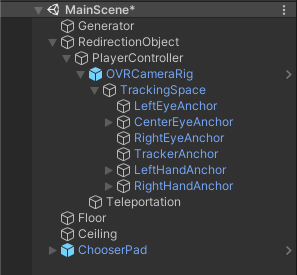
\includegraphics[width=0.5\textwidth]{images/hierarchy.png}
    \caption{Die Hierachie der Unity-Szene vor der Laufzeit}\label{figure:hierarchy}
\end{figure}

Das \textquote{Generator}-Objekt existiert um die Scripts, die ihm als Komponenten %de en?
angehängt sind in die Szene zu integrieren, sodass diese ausgeführt werden. Darauf folgt das \textquote{RedirectionObject}, welches, als effektiver Parent des \textquote{OVRCameraRig} später dafür genutzt wird, die Rotationgains auszuführen. Zwischen diesen beiden Objekten liegt aber noch der PlayerController. Dieser wird in den beiden Kontrollbedingung für die Fortbewegungsarten genutzt.

Das \textquote{OVRCameraRig} und die hierarchisch untergeordneten Elemente sind ein vom Oculus Integration SDK bereitgestelltes Prefab, es integriert die Funktionalität der virtuellen Umgebung in die Unity-Szene.

\textquote{Floor} und \textquote{Ceiling} repräsentieren Boden und Decke der Szene. Das zuletzt in \autoref{figure:hierarchy} dargestellte Objekt ist das \textquote{ChooserPad}. Dies ist ein, den später beschriebenen Nummerneingabefeldern nachempfundener Mechanismus mit dem die Nutzer:in später einstellen kann, welche der Testbedingungen sie ausführen möchte. Dies wird genauer in \autoref{sec:chooserpad} erklärt.

%TODO: hierarchy zur laufzeit figure + kleiner text + bild


\section{Design der Szene} \label{sec:scene-design}
%TODO: Bild von Raum
Im folgenden werde ich die Designentscheidungen, die die Optik der Szene bestimmen erläutern.

Die virtuelle Umgebung, die die Nutzer:in durchschreitet ist der eines Dungeons nachempfunden. Dies ist in Computerspielen ein häufig eingesetztes Setting, weltbekannte Spiele wie
\textquote{The Elder Scrolls V: Skyrim}, %TODO: sources?
die \textquote{Final Fantasy} Spielreihe,
die \textquote{The Legend of Zelda} Spielreihe,
und besonders sogenannte \textquote{Roguelike}-Spiele, wie
die \textquote{Diablo} Spielreihe,
\textquote{The Binding of Isaac},
oder \textquote{Darkest Dungeon}, beinhalten alle zumindest zum Teil Dungeonartige Level, die den Spieler herausfordern eine dunkle Umgebung zu erkunden und gegen fiese Gegner zu kämpfen.
Obgleich letzteres in den hier erzeugten Leveln nicht vorkommt, ist das  Ambiente bewusst ein wenig düster gehalten und erinnert optisch an einen Dungeon. Sehr hilfreich ist dafür die aus dem Unity-Asset-Store heruntergeladene Textur \cite{dungeon-material}, die die Wände schmückt und ihnen ein rustikales, dungeonartiges Gefühl verleihen.

%grafik von rogue?
Das Spiel \textquote{Rogue}, von 1980, nachdem auch das Genre \textquote{Roguelike} benannt wurde ist ein Meilenstein in der Prozeduralen Levelgeneration gewesen und hat bis heute großen Einfluss auf die Welt der Computerspiele. Auch dabei geht es darum einen Dungeon zu erkunden, auch wenn dieser verständlicherweise graphisch, noch nicht besonders aufbereitet gewesen ist.

Abgesehen davon bietet die Umgebung eines Dungeons viele Freiheiten, was den Realismus der Welt angeht. Es wird nicht hinterfragt wieso ein Gebäude so strukturiert sein sollte, dass man die ganze Zeit um die Ecke geht oder wieso die Türen sich öffnen und schließen, in dem sie magisch erscheinen oder sich auflösen.

Um die Erkundungsstimmung noch ein wenig zu verstärken und eine realistische Lichtquelle in die Welt einzubauen trägt die Nutzer:in eine Kopflampe, dies ist ein einfacher Spotlight mit leicht bläulichem Licht, dessen Parent die Kamera des Spieler:innenavatars ist.

%MCI mässige quellen wären hier gut

\section{Virtueller Avatar}
Um die Nutzer:in in der Szene zu repräsentieren und ihr die Möglichkeit zu geben mit dieser zu interagieren kann sie über die Tranformation von Datenbrille und Controller einen virtuelle Avatar steuern. Auf diese Weise ist es ihr möglich mithilfe der Hände dieses virtuellen Avatars die Knöpfe von Nummerneingabefeldern zu bestätigen und in der später beschriebenen Teleportationsbedingung den Ort auszuwählen zu dem sie sich teleportieren möchte. Die virtuellen Hände folgen der Bewegung und Drehung, und sogar der Stellung der Finger, der echten Händer von der Nutzer:in solange sie die Oculus Controller auf die richtige Weise hält. Auch mit ihrem Kopf kann die Nutzer:in mit der Szene interagieren, auch Knöpfe betätigen, wenngleich dies auch eine weniger Hilfreiche Funktionalität ist.

Diese Funktionalität wurde vom Oculus SDK bereit gestellt und wurde von mir lediglich in die Szene integriert. %quelle?
Damit virtuelle Objekte innerhalb der Szene dem realen Körper der Nutzer:in folgen wurden diese hierarchisch den dafür bereit gestellten \textquote{Anchor}-Objekten unterstellt (siehe \autoref{figure:hierarchy}). Für die Hände wurden dafür die vom Oculus SDK bereiten gestellten Prefabs genutzt. %name of prefabs
An den \textquote{CenterEyeAnchor} wurde die in \textquote{sec:scene-design} erwähnte Kopflampe angehangen, sodass diese der Blickrichtung der Nutzer:in folgt.

\section{Implementierung der Rotationgains}

Die Umsetzung der Rotaiongains erfolgt mithilfe des
%TODO: Von wem genau kommt space extender? quelle
freundlicherweise zur Verfügung gestelltem Unity-Package \textquote{Space-Extender}. Dieses bietet das Prefab \textquote{RotationRedirector}, welches im Code instanziiert werden kann und dann nachdem es richtig positioniert ist, die Dimensionen des Trackingspaces und den virtuellen Avatar der Nutzer:in und die Kooridinaten, des Punktes, um den rotiert werden soll übergeben bekommen hat, dazu in der Lage ist einen Rotationgain auf die Nutzer:in anzuwenden. Der RotationRedirector wird nachdem das alles geschehen ist für jeden Raum, an die Instanz des RotationGainMechanism, die für eben jenen Raum zuständig ist übergeben, sodass er aktiviert werden kann sobald das Signal vom entsprechenden Collider kommt, dass die Nutzer:in sich über dem Rotationspunkt ($\vec{P}$) befindet.
%TODO: wie stark sind die rotation gains und wann wie doll wieviel grad etc #unitydata


%impossible spaces
\section{Fortbewegungsarten}
%TODO:implementierung joystick mit daten
\subsection{Joystick-Steuerung} \label{subsec:joystick-implementation}
%TODO:implementierung teleport mit daten
    %TODO: technische Daten über joysticks: geschwindigkeit, beschleunigung, in blickrichtung etc(?).
    Die Joystick-Fortbewegung wurde mithilfe einiger, vom Oculus Integration SDK gelieferter Scripts, hauptsächlich dem \textquote{OVRPlayerController} umgesetzt. Dieser befindet sich dann auf dem in \autoref{sec:hierarchy} beschriebenen PlayerController und steuert so diesen und dessen Kindelemente, so auch den virtuellen Avatar der Nutzer:in.
\subsection{Teleportierung}
    Auch diese Bedingung wird mithilfe einiger, mit dem Oculus Integration SDK gelieferten Scripts, das auf dem PlayerController liegt, implementiert. Hierbei ist hauptsächlich das \textquote{} %TODO: feddich machen
\subsection{Real-Walking}

\section{Der Rotationgain Inzentivierungs Mechanismus}
\label{sec:rotgaininc}

Damit der Rotationgain seinen Effekt erzielen kann ist es wichtig, dass die Nutzer:in sich ungefähr auf den Punkt $\vec{P}$ stellt und ihren Kopf um die Y-Achse dreht.
Damit sich dies intuitiver anfühlt und die Aufmerksamkeit nicht so konkret auf den Rotationgain gelenkt wird, habe ich mich dagegen entschieden den Nutzer:innen einfach den Punkt $\vec{P}$ zu markieren und sie zu bitten dort ihren Kopf zu drehen, sondern habe mir einen Vorwand ausgedacht, wieso es zum einen Notwendig ist an der Stelle zu stehen und zum anderen, wieso sie ihren Kopf drehen müssen.

%TODO: NumPad Picture
Um diesen Effekt zu erzielen wird ein Nummern-Eingabefeld, an der Korridorinnenwand in Richtung des Raumes aus dem die Nutzer:in gerade kommt, genau vor die Position $\vec{P}$ plaziert. In dieses Eingabefeld sollen dann mehrere zweistellige Nummern, die am anderen Ende des Korridors, auf einer digitalen Tafel angezeigt werden eingegeben werden, bis die Tür sich öffnet. Auf der Tafel wird nur eine zweistellige Nummer zur Zeit angezeigt.
Dies sorgt dann sowohl dafür dass die Nutzer:in sich automatisch auf den Punkt $\vec{P}$ stellt, um möglichst gut die Nummern eingeben zu können, als auch dafür, dass die Nutzer:in ihren Kopf wiederholt um die Y-Achse dreht weil sie abwechselnd ablesen muss welche Zahlen auf der Tafel hinter ihr angezeigt werden und dann die Zahlen in das Eingabefeld schräg vor ihr eingeben muss. Dies sorgt für einen intuitiven Grund den Kopf zu drehen und somit dafür den Rotationgain zu nutzen. Wenn der Fortschritt des Rotation-Gains abgeschlossen ist und ein weiteres Mal die korrekte Nummer in das Eingabefeld eingegeben wurde, öffnet sich die Tür vor der Nutzer:in (also die \textquote{Seitentür}) sodass die Nutzer:in in den nächsten Raum gehen kann. Da nun der Trackingspace genau den nächsten Raum umgibt ist es wichtig, dass die Nutzer:in nicht versucht zurück in den vorherigen Raum zu gehen. Aus diesem Grund schließt sich hinter der Nutzer:in eine vorher noch nicht zu erkennenende Tür.

Im Programm-Code findet sich dieser ganze Vorgang in der Klasse \textquote{RotationGainMechanism}. Dieser wird für jeden Raum erstellt und auch dem Objekt des Raumes als Component hinzugefügt. Eine Instanz des RotationGainMechanisms ist also immer für den Raum zuständig auf dem er sich befindet. Mit der \textquote{Init}-Funktion wird das Objekt direkt nach der Erstellung initialisiert, hier meldet sich die Instanz dann auch in der zugehörigen Eingabefeld-Klasse (\textquote{NumPadScript}) als Observer an. Sobald sich die Nutzer:in dann in den um die Position $\vec{P}$ herum platzierten Collider wird mit der Funktion \textquote{StartMechanism} die Prozedur gestartet. Zunächst wird eine neue zweistellige Zahl mithilfe des (von Unity bereitgestellten) Pseudozufallgenerators erstellt, dann wird diese Zahl auf der dem aktuellen Raum zugehörigen Tafel angezeigt. Sobald die Bestätigungstaste des Eingabefelds gedrückt wurde (\textquote{$\#$}), wird überprüft ob der Fortschritt des Rotation-Gains schon bei 100\% ist. Falls nicht, beginnt das ganze von vorne und es wird eine neue Zahl erstellt. Wenn der Rotation-Gain vollständig abgeschlossen ist (also eine 90\textdegree\ Drehung stattgefunden hat) wird dem \textquote{RoomAndProgressManager} mitgeteilt dass der aktuelle Raum abgeschlossen ist und die Tür öffnet sich.

In den Kontrollbedingungen wird kein Rotationgain angewandt. Dennoch müssen die Proband:innen auch hier Zahlen in das Eingabefeld eingeben. In diesen Szenarien wird die Türöffnung aus offensichtlichen Gründen nicht von der vervollständigung des Rotationgains abhängig gemacht, sondern wird eine Zufallszahl zwischen 4 und 8 bestimmt und mitgezählt, wie oft Zahlen bestätigt wurden. Wenn die Zufallszahl erreicht wird öffnet sich die Tür. Durch Erfahrungen beim Testen hat sich gezeigt dass es etwa zwischen 4 und 8 Eingaben bedarf, bevor der Rotationgain abgeschlossen ist.

\section{Bedingungsauwahl und Laden der Szene} \label{sec:chooserpad}
%image chooserpad
\begin{figure}[!h]

    \caption{ChooserPad caption}\label{figure:chooserpad}
\end{figure}
Damit die Versuchspersonen der später vorgestellten Studie die Level mit den unterschiedlichen Bedingungen ausführen können, gibt es ein Menü, in dem diese Ausgewählt werden können. Darin befindet sich nur der Boden, die Decke und das Bedingungsauswahlfeld (siehe \autoref{figure:chooserpad}). Auf diesem kann die Nutzer:in auf einem $3 \times 3$ Eingabefeld auswählen, welche Versuchsbedingung sie starten möchte. In der späteren Studie wird vorgegeben, welche die Proband:in auswählen soll. Die einzelnen Bedingungen sind folgendermaßen kodiert. $A$ steht für die Real-Walking Fortbewegungsart-Bedingungen, $B$ für Joystick-Steuerung, $C$ für Teleportation, $1$ für eine Raumanzahl von 3 Räumen, $2$ für 6 und $3$ für 9 Räume. Die Auswahl erfolgt per Tastendruck, allerdings wird das Level erst generiert und gestartet, sobald anschließend die Bestätigungstaste \# gedrückt wird.

Das ganze funktioniert dann so, dass die Instanz der \textquote{SceneLoader}-Klasse, die auf dem \textquote{Generator}-Objekt liegt, eine Instanz auf das Auswahlfeld und auf die \textquote{GenerateLevel}-Instanz hält. Sobald die Bestätigungstaste gedrückt wurde, werden die entsprechenden Einstellungen daran vorgenommen, einige VR-Einstellungen getätigt (beispielsweise das Deaktivieren, der Reset-Möglichkeit, die bei der Real-Walking Bedingung zu Problemen führen könnte), die Fortbewegungsart festgelegt, indem die entsprechenden Components, die die Joysticksteuerung oder die Teleportation ermöglichen (siehe %link
) aktiviert, oder deaktiviert werden und zu guter letzt die Teleportierung der Nurtzer:in in den ersten Raum des Levels getätigt.

\section{Messmechanismen und Datenspeicherung} \label{sec:measure-distance}
Um an späterer Stelle einschätzen zu können, wie gut die Proband:innen die Entfernung die sie sich fortbewegt haben geschätzt haben ist es notwendig eben dies auch zu messen. Zusätzlich dazu ist es auch notwendig diese Daten zu speichern. Im folgenden werde ich erläutern, wie dies implementiert ist.

Da es nicht darum geht die Luftlinie zwischen Start und Ende des Levels zu messen, da dann die Bewegungsweise der Proband:in keine Rolle mehr spielen würde, sondern ihre konkreten Fortbewegungsstrecke zu messen, ist diese Aufgabe nicht gänzlich trivial. Würde man einfach in jedem Tick die Kopfposition des virtuellen Avatars der Proband:in speichern, die Distanz zum vorherigen Punkt berechnen und aufsummieren, wäre das Ergebnis sehr ungenau. %?
Da nun jede millimeterbewegung des Kopfes aufsummiert werden würde, würde eine einfache Kopfdrehung die fortbewegte Strecke schon um einen großen Teil erhöhen. Dies würde dazuführen, dass die Messung der fortbewegten Strecke nicht mehr intuitiv einzuschätzen wäre.

Um dem entgegenzuwirken habe ich die Auflösung dieser Messung deutlich veringert, indem nicht mehr jedes Frame, diesen Prozess durchläuft, sondern nur ein Frame etwa alle 2 Sekunden. So werden deutlich grobere Bewegungen gemessen und die gemessenen Ergebnisse passen deutlich besser zu der intuitiven Einschätzung der Entfernung.
%TODO: zu unwissenschaftlich? nochmal best practices recherchieren %einfach noch mehr dazu sagen dann geht das schon

All dies ist im \textquote{RoomAndProgressManager} implementiert. Hier gibt es eine \textquote{StartTimeMeasure}-Methode, die zum Start der Bedingung vom \textquote{SceneLoader} aufgerufen wird und eine \textquote{AddDistance}-Methode, die in der von der \textquote{Update}-Methode alle 150 Frames einmal aufgerufen wird. Diese bestimmt dann euklidisch die Distanz zwischen der aktuellen Position der Nutzer:in und der zuletzt gemessenen und addiert diese auf eine Kummulationsvariable.

Sobald das Level der Versuchsbedingung abgeschlossen ist wird diese Kummulationsvariable an den \textquote{FirebaseHandler} weitergeleitet, der nun die Daten der aktuellen Versuchsbedingung an die private Datenbank sendet um die Daten für die spätere Auswertung zu speichern.

\chapter{Levelgenerierung}
\label{section:generate}
Dieses Kapitel beschreibt, wie genau die Generierung eines in diesem Projekt genutzen Levels funktioniert. Nacheinander werde ich die grundlegenden Ideen hinter der Levelgenerierung erörtern und dabei jeweils genauer auf ihre Implementierung eingehen um dann den Algorithmus, der die unterschiedlichen Codeblöcke nutzt um die Levelstruktur zu generieren, zu beschreiben und vorzustellen.
Zuerst wird besprochen, wie die Räume angeordnet werden müssen damit sie durch den Rotation-Gain verbunden werden können. Dann wird erklärt und vorgestellt wie die Korridore, die in den Räumen generiert werden um der Nutzer:in einen klaren Weg voran zu präsentieren und den Übergang zwischen den Räumen intuitiver zu gestalten, erstellt werden. Als nächstes beschreibe ich die Vorgänge die für die Generierung der Wände der Räume verantwortlich sind und erkläre wie die entsprechenden Berechnungen stattfinden.
Um hinterher dann den Generierungs-Algorithmus und den zugehörigen Quelltext vorzustellen wird dann noch Beschrieben an welchen Stellschrauben manipuliert werden kann um heterogene Ergebnisse zu bekommen, erst hier können (Pseudo-)Zufallsfaktoren eine Rolle spielen.
Den krönenden Abschluss dieses Kapitel bekommt dann der Abschnitt,
der die Zusammensetzung des Algorithmusses zunächst erklärt und den entsprechenden Quelltext dann auch noch ausführlich vorstellt.

\section{Raumplatzierung}

Um zu verstehen wie die Berechnung der Ecken eines Raumes funktioniert ist es zunächst essentiell, die Grundidee hinter der Raumanordnung zu verstehen.

\begin{figure}[H]
    \ctikzfig{2rooms_a}
    \caption{Veranschaulichung der Raumstellung zueinander, sodass $\vec{P}$ den Drehpunkt kennzeichnet }\label{figure:two_rooms} %TODO: formulierung
    %TODO: P Point size, vec
\end{figure}

%paragraph Erklärung
\subsection{Grundidee}
\label{subsec:roomplaceidea}
%Um die durchgehende Weiterführung des Levels zu ermöglichen werden zwei Räume immer genau so angeordnet, dass ein Rotation-Gain, der genau bis zu einer Verdrehung der beiden Realitäten von 90\textdegree\ angewandt wird, während die Nutzer:in an einem bestimmten Punkt in der Ecke des Raumes steht,
Wenn ein Rotation-Gain angewandt wird verdrehen sich virtuelle und reale Realität umeinander, um einen konkreten Drehpunkt. In der Regel stellt dieser die Position der Nutzer:in dar, damit der Effekt allerdings genau plan- und vorhersagbar ist findet die Drehung der Umgebung nicht, wie sonst in VR üblich um den Kopf der Nutzer:in, sondern um einen bestimmten vordefinierten Punkt $\vec{P}$ statt.

Wenn diese Position $\vec{P}$ sich in einer Ecke des (rechteckigen) Trackingspace-Raumes befindet, zudem genau gleich weit von beiden Wänden, die diese Ecke bilden, entfernt ist und dann ein gerichteter Rotationgain angewandt wird,
bis genau 90\textdegree\ Verdrehung erreicht sind, dann steht der aktuelle begehbare Bereich in der virtuellen Umgebung $B$, dem vorherigen begehbaren virtuellen Bereich, der ebenfalls durch den Trackingspace definiert war $A$, genau orthogonal gegenüber.

Vorher hat der Bereich $A$ genau den virtuellen Bereich innerhalb des Trackingspaces dargestellt. Die beiden Areale $A$ und $B$ überlappen sich zwar in einem gewissen Bereich, in dem die Nutzer:in nach Beendigung des Rotationgains dann auch gerade steht $O$, aber ein Großteil von $A$ ist nun Teil des Bereiches der virtuellen Umgebung geworden der, begrenzt durch den Trackingspace, nicht zugänglich ist. Auf diese Weise ist also für die Nutzer:in ein neuer Bereich der virtuellen Umgebung begehbar geworden.
Wenn der Rotationgain subtil genug angewandt wurde hat die Nutzer:in(Idealerweise) nicht bewusst wahrgenommen, dass die Welten sich verdreht haben. Wenn sie nun also geradeaus geht entsteht der Eindruck, dass nun ein weiterer Teil der Welt zugänglich geworden ist.

Ziel des Algorithmus ist es eine Reihe von aufeinander folgenden Räumen zu generieren, sodass die Nutzer:in sich durch ein Dungeon-artiges Level bewegen kann um vom ersten zum letzten Raum zu gelangen.
Die Grundidee hinter der Raumgenerierung ist es also, dass genau die beiden Areale $A$ und $B$ von Wänden umgeben werden. %TODO: formulierung
In \autoref{figure:two_rooms} wird ersichtlich, wie die beiden Räume zueinander Stehen müssen um diesen Effekt zu ermöglichen.

Um dann also von Raum $A$ zu Raum $B$ zu kommen muss die Nutzer:in sich an der Position $\vec{P}$ oft genug drehen und ein Rotation-Gain bis zu 90\textdegree\ in die jeweilige Richtung angewandt werden. Bei dem Beispiel in \autoref{figure:two_rooms} muss der Rotationgain bei Yaw-Kopfdrehungen nach links positiv und nach rechts negativ verlaufen um den gewünschten Effekt möglichst Effizient zu erzielen. Andersherum wäre auch möglich, dann müssten sich die Welten aber nicht um
90 \textdegree sondern um 270 \textdegree
drehen.

Danach kann sie mit der Illusion geradeaus zu gehen einen neuen Raum erkunden während sie sich eigentlich nur weiter innerhalb des realen Trackingspaces bewegt. Der reale Trackingspace umschließt bei der hier vorgestellten Methode also immer genau den Raum in dem sich die Nutzer:in gerade befindet.

\subsection{Berechnung der Ecken}
\label{subsection:calccorners}

\begin{figure}[H]
    \centering
    \begin{tikzpicture}
	\begin{pgfonlayer}{nodelayer}
		\node [style=none] (37) at (-7, 7) {};
		\node [style=none] (38) at (1, 7) {};
		\node [style=none] (39) at (-7, -3) {};
		\node [style=none] (40) at (1, -3) {};
		\node [style=none] (41) at (-1, 7) {};
		\node [style=none] (42) at (9, 7) {};
		\node [style=none] (43) at (-1, -1) {};
		\node [style=none] (44) at (9, -1) {};
		\node [style=none] (0) at (0, 7) {};
		\node [style=none] (18) at (9, -1) {};
		\node [style=none] (19) at (-1, -1) {};
		\node [style=none] (20) at (9, 7) {};
		\node [style=none] (21) at (-1, 7) {};
		\node [style=none] (45) at (-1, 6) {};
		\node [style=none] (47) at (-1, 6) {};
		\node [style=none] (50) at (0.25, 6.5) {$dP$};
		\node [style=none] (51) at (-0.5, 5.75) {$dP$};
		\node [style=none] (52) at (0, 6) {};
		\node [style=none] (53) at (0.25, 5.75) {$P$};
		\node [style=none] (55) at (-1.25, 6) {$cP$};
		\node [style=none] (57) at (9, 7.25) {$C_b$};
		\node [style=none] (58) at (-1, 7.25) {$C_a$};
		\node [style=none] (59) at (-1, -1.25) {$C_d$};
		\node [style=none] (60) at (9, -1.25) {$C_c$};
	\end{pgfonlayer}
	\begin{pgfonlayer}{edgelayer}
		\draw [style=new edge style 0] (40.center)
			 to (39.center)
			 to (37.center)
			 to (38.center)
			 to cycle;
		\draw [style=new edge style 1] (43.center)
			 to (41.center)
			 to (42.center)
			 to (44.center)
			 to cycle;
		\draw [style=arrow] (21.center) to (47.center);
		\draw [style=arrow] (19.center) to (47.center);
		\draw [style=arrow] (18.center) to (19.center);
		\draw [style=arrow] (20.center) to (21.center);
		\draw [style=dashes] (52.center) to (0.center);
		\draw [style=arrow] (45.center) to (52.center);
        \draw [decorate,decoration={brace,mirror,amplitude=10pt}](-1,-1.5) -- (9,-1.5) node [midway,yshift=-0.25in] {$length$};
        \draw [decorate,decoration={brace,amplitude=10pt}](-1.5,-1) -- (-1.5,7) node [midway,xshift=-0.40in] {$width$};
	\end{pgfonlayer}
\end{tikzpicture}

    \caption{Zur Eckenberechnung genutzte Vektoren. Mit $\vec{C_0}, \vec{C_1}, \vec{C_2}, \vec{C_3}$ werden die Ecken bezeichnet, mit $S_{0}, ...,  S_3$ die Seiten des Raumes (Nicht die zur Eckenberechnung genutzen Vektoren). } %TODO: bessere caption, was für eine scheisse
    \label{figure:calculateCornersFig}
\end{figure}

Der Effekt, dass die Räume in denen sich die Nutzer:innen gerade befinden, immer genau den Trackingspace darstellen wird zu großen Teilen duch die besondere Art der Raumgenerierung ermöglicht. Diese möchte ich im folgenden Vorstellen.

Zunächst müssen die Koordinaten der Ecken innerhalb der virtuellen Umgebung bestimmt werden. Für den ersten Raum ist es nicht schwierig, die virtuellen Koordinaten der Ecken der Trackingspace-Boundaries werden vom Oculus Integration SDK geliefert.
In der \textquote{GeneratorOculusInterface} Klasse werden diese zu Beginn der Levelgenerierung abgefragt und der \textquote{GenerateLevel}-Klasse zur Verfügung gestellt. Um allerdings die Raumecken der folgenden Räume zu bestimmen müssen einige Punkte, Längen und Vektoren bereits definiert oder errechnet worden sein. Wie diese zustande kommen wird im darauf folgenden Absatz erläutert. Für alle Räume, außer dem ersten berechnen sich die Eckkoordinaten, dann folgendermaßen.

% $$ cP = P + (-1) * sDD * dP $$

% $$ C_a = cP + (-1) * btF * dP $$
% $$ C_b = C_a + sDD * length $$
% $$ C_c = C_d + sDD * length $$
% $$ C_d = cP + btF * (width - dP) $$
%TODO: nochmal checken

    \begin{align}
        \begin{split}\label{eq:1}
            \vec{cP} ={}& \vec{P} + (-1) * \vec{sDD} * dP
        \end{split}\\ \\
        \begin{split}\label{eq:2}
            \vec{C_0} ={}& \vec{cP} + (-1) * \vec{btF} * dP
        \end{split}\\
        \begin{split}\label{eq:3}
            \vec{C_1} ={}& \vec{C_0} + \vec{sDD} * length
        \end{split}\\
        \begin{split}\label{eq:4}
            \vec{C_2} ={}& \vec{C_3} + \vec{sDD} * length
        \end{split}\\
            \vec{C_3} ={}& \vec{cP} + \vec{btF} * (width - dP)\label{eq:5}
        \end{align}

    % \begin{align}
    %     \begin{split}\label{eq:1}
    %         a ={}& b + c + d\\
    %              & + e + f + g
    %     \end{split}\\
    %     \begin{split}\label{eq:2}
    %         k ={}& l + m + n + m + n + m + n\\
    %              & + o + p + q
    %     \end{split}\\
    %         r ={}& s + t (u + v + w)\label{eq:3}
    %     \end{align}
Auch zu sehen ist diese Berechnung in dem in der \autoref{figure:calculateNewCornersScript} gezeigen Quelltext.
Wie die hier genutzen Variablen $\vec{cP}$, $\hat{sDD}$, $\hat{btF}$, $width$ und $length$ definiert sind wird aus \autoref{figure:calculateCornersFig} ersichtlich. %TODO: figure erweitern
        %weiteres dP nach rechts
        %sDD
        %btF
$\vec{cP}$ steht dabei für den Punkt hinter $\vec{P}$, der genau eine $dP$-Länge in Richtung des alten Raumes liegt. $\hat{sDD}$ (sideDoorDirection) ist ein normalisierter Richtungsvektor,
der die Richtung des Korridors des letzen Raumes erweitert. %TODO: besser beschreiben, hier weiss man noch nicht was ein korridor ist
$\hat{btF}$ (backToFront) ist auch ein normalisierter Richtungsvektor, der orthogonal zu $\hat{sDD}$ steht.
Er zeigt von der hinteren Wand des Korridors des vorherigen Raumes zur vorderen Wand. %TODO: hier auch
Diese Richtungsvektoren werden vor der Eckenberechnung errechnet indem die Vektoren, die die entsprechenden Ecken des schon bestehenden Raumes darstellen, voneinander subtrahiert werden um die gemeinten Richtungen in Form von Vektoren zu errechnen, bevor sie dann normalisiert werden.

$width$ beschreibt die Breite der Räume, während $length$ die Länge beschreibt. Diese beiden Variablen hängen von den Maßen des ersten Raumes ab, bei dem die Eckkoordinaten ja den Trackingspace der Nutzer:in abbilden. Wichtig ist noch zu erwähnen, dass die in der eben erwähnten Abbildung gezeigte Folge von Ecken und Seiten, nicht genau spiegelverkehrt ist wenn der Raum in die andere Richtung generiert würde (siehe \autoref{sec:random}), sondern die Reihenfolge der Ecken genau invertiert läuft. Das ganze ist also nicht nur vertikal, sondern auch horizontal gespiegelt zu der Darstellung in \autoref{figure:calculateCornersFig}.

\begin{figure}[H]%TODO: frisieren und kommentieren
    \centering
    \sourcecode{calculateNewCorners.cs}
    \caption{Funktion zur Berechnung der virtuellen Eckkoordinaten des nächsten Raumes}
    \label{figure:calculateNewCornersScript}
\end{figure}

\section{Korridore}
\label{sec:corridor}
%paragraph Erklärung
%TODO: Bild eines Korridors
Damit die Nutzer:in versteht wie sie in den nächsten Raum kommt sind die Räume so gestaltet, dass es einen offensichtlichen Weg voran gibt. Um dies zu erreichen wird in die Räume jeweils ein Korridor, also ein kleiner Flur, der auf die Tür zum nächsten Raum zuläuft, generiert. In der hier vorgestellten Implementierung der Levelgenerierungmethode wird der Korridor für jeden Raum generiert, bevor mit der Eckenberechnung für den nächsten Raum begonnen wird, und wie in \autoref{sec:random} beschrieben wird, hängt diese sogar von dem Korridor ab. Sie sind also wichtiger Bestandteil dieser Implementierung, die Levelgenerierungmethode ließe sich aber auch ohne sie realisieren. In diesem Abschnitt wird die Generierung dieser Korridore für ihre jeweiligen Räume erläutert.

Zunächst wird eine Kante des Grundecks des Raumes ausgewählt, an der ein Korridor erstellt wird (diese wird Pseudozufällig ausgewählt, siehe \autoref{sec:random}). Er kann sowohl an einer kürzeren Kante als auch an einer längeren Kante des Grundecks des Raumes erstellt werden, nur nicht an der Seite an der das Ende des Korridors des vorherigen Raums herausragt, da sich die beiden Korridore sonst kreuzen würden.

Der Korridor hat zwei Türen: Eine \textquote{Haupttür}, durch die die Nutzer:in in den Korridor hineinkommt und eine \textquote{Seitentür}, die anfangs noch verschlossen ist und in den nächsten Raum führt. %optional todo: figure mit korridor aus topansicht

In diesem Korridor werden dann Elemente platziert die gemeinsam für einen Mechanismus sorgen, der die Nutzer:in inzentiviert sich genug um die $Yaw$-Achse zu drehen, dass die wirkliche und die virtuelle Realität sich dank des Rotationgains genug umeinander drehen, dass der nächste Raum nun mit dem realen Tracking-Space übereinstimmt. Dieser Mechanismus wird in
\autoref{sec:rotgaininc}
genauer beschrieben.

\subsection{Korridor-Meshgenerierung}
\label{subsec:corridormesh}
Um einen solchen Korridor zu generieren müssen zunächst die Koordinaten der  für das Korridor-Mesh genutzten Knotenpunkte (Vertices) bestimmt werden. Zudem müssen dann entsprechende Flächen (Faces) gespannt und für jeden Knotenpunkt dann auch die UV-Koordinaten errechnet werden, sodass die Korridore texturiert werden können. All dies geschieht in der \textquote{RoomGenerator}-Klasse.

Ein Korridor besteht aus einem Boden, einer Frontalwand, zwei Seitenwänden und einer Rückwand. Zudem sind in der Frontalwand und einer der Seitenwände Türen eingelassen.
Bevor die Meshgenerierung stattfinden kann muss zunächst die Türposition auf der Frontalachse, $D$, bestimmt werden. Dabei handelt es sich um einen Wert zwischen $0$ und $1$, der für jeden Raum (Pseudo-)zufällig generiert wird (siehe \autoref{sec:random}). Mit diesem Wert wird die Frontal-Türposition bestimmt, je geringer er ist desto weiter links liegt die Haupttür in der Frontalwand. Ist der Wert geringer als 0.5 befindet sich die Seitentür in der rechten Seitenwand, sonst in der linken, sodass diese immer auf der gegenüberliegende Seite der Haupttür liegt.

Es gibt zwei Möglichkeiten der Struktur einer Wand, abhängig davon ob in ihr eine Tür eingelassen ist oder nicht. Der simplere Fall trifft zu wenn in der Wand keine Tür liegt, dann besteht die Wand aus einem Quader, also aus 8 Vertices.
Die Wandstruktur der Türbeinhaltenden Alternative wird in \autoref{figure:doorCalcFig}
veranschauligt. Dabei ist allerdings zu beachten, dass nur die Frontalansicht auf eine solche Wand gezeigt ist, die Innenseite derselben Wand hat die selbe Struktur. Zudem sind die frontalen Vertices der Tür jeweils mit ihren inneren Gegenspielern durch Faces verbunden, sodass man beim durchschreiten der Tür nicht ins innere der Wand blicken kann.

\paragraph*{Vertices}

Das Generieren eines solchen Korridors läuft dann also wie folgt ab. Gegeben sind die die Eckkoordinaten des Raumes in den der Korridor platziert werden soll ($\vec{C_0}, ..., \vec{C_3}$), diese werden wie in \autoref{subsection:calccorners} berechnet, die Seite des Raumes, an der der Korridor liegen soll ($S_s$) und die Türposition $D$, welche mithilfe eines Pseudo-Zufallsalgorithmus ermittelt werden (siehe \autoref{sec:random}). Dazu noch einige Werte, die im vorhinein von der Gestalter:in der Level vordefiniert werden: Die Tiefe des Korridors $d$, durch die sich auch der in \autoref{subsection:calccorners} besprochene Wert $dP$ also der Abstand des Punktes $\vec{P}$ zu den Wänden der Ecke des Raumes ergibt: $dP = \frac{d}{2}$, die Höhe $h$ und Dicke der Wände $w$ sowie die Höhe ($dh$) und Breite ($dw$) der Tür.

Als erstes werden die unteren, äußeren Punkte berechnet. ($\vec{F_0}, ..., \vec{F_3}$)
Dabei wird mit den beiden hinteren, äußeren Punkten des Korridors begonnen. Da die Ecken eines Raumes immer im Uhrzeigersinn gespeichert werden lassen sich diese Punkte heraussuchen indem die $s$'te Ecke des Raumes und die im Uhrzeigersinn darauf folgende auswählt werden. %TODO: formulierung

$$ \vec{F_0} = \vec{C_s} $$
$$ \vec{F_1} = \vec{C_{((s+1)\pmod 4)}} $$

Damit wird der Richtungsvektor $\hat{rTL}$ (rightToLeft) errechnet indem die rechte Ecke von der linken Ecke subtrahiert wird und das Ergebnis dann normalisiert wird.
%TODO: all previous points and vectors need to use \vec
$$ \vec{rTL} = \vec{F_1} - \vec{F_0} $$ %TODO: normalisieren?
$$ \hat{rTL}=\frac{\vec{rTL}}{\left | \vec{rTL} \right |} $$

Um die beiden vorderen äußeren Ecken zu bestimmen muss nun ein Richtungsvektor $\hat{tF}$ (toFrontWall) berechnet werden der von der Seite $S_s$ in Richtung der gegenüber liegenden Seite des Raumes zeigt. Hierfür wird das Kreuzprodukt von $\hat{rTL}$ und dem nach oben gerichteten Einheitsvektor berechnet und das Ergebnis normalisiert.

$$ \hat{up} = \begin{pmatrix} 0 \\ 1 \\ 0 \\ \end{pmatrix} $$
$$ \vec{tF} = \hat{rTL} \times \hat{up} $$ %TODO: oben vektor, kreuzprodukt, normalisieren
$$ \hat{tF} = \frac{\vec{tF}}{\left | \vec{tF} \right |} $$

Um nun die vorderen Punkte zu bestimmen wird einfach der neue Richtungsvektor $\hat{tF}$ mit $2 * dP$ multipliziert und auf die hinteren Punkte addiert.

$$ \vec{F_2} = \vec{F_0} + \hat{tF} * dP $$
$$ \vec{F_3} = \vec{F_1} + \hat{tF} * dP $$

Nach dem nun klar gewordenen Prinzip, die Knotenpunkte zu berechnen indem schon errechnete Knotenpunkte mit den entprechenden Richtungsvektoren multipliziert werden lassen sich nun die äußeren, oberen Ecken des Korridors bestimmen, hierfür werden die unteren Ecken mit dem Vektor $\vec{T}$ addiert, der sich wie folgt berechnet:

$$\vec{T} = \hat{up} * h $$ %TODO: up

$$ \vec{F_4}, ..., \vec{F_7} = \vec{F_0} * \vec{T}, ..., \vec{F_3} * \vec{T} $$ %TODO: is multiplication with the * actually acurate?

Um die inneren Punkte zu berechnen werden die äußeren Ecken nach dem selben Prinzip, jeweils mit den entsprechenden Richtungsvektoren, die dann mit $w$ multipliziert werden addiert. Die inneren Punkte liegen mit den äußeren Punkten auf einer Höhe. Die linken Ecken werden also jeweils nach rechts addiert, die rechten nach links, die hinteren nach vorne, die vorderen nach hinten, sodass jede innere Ecke mit zwei $w$-langen Vektoren von den Äußeren in Richtung der Mitte verschoben wurde. Für die Richtung nach rechts wird $\hat{rTL}$ verwendet, nach links $\hat{rTL} * (-1)$, nach vorne $\hat{tF}$ und nach hinten $\hat{tF} * (-1)$.

\begin{figure}[H]
    \centering
    \begin{tikzpicture}
	\begin{pgfonlayer}{nodelayer}
		\node [style=none] (0) at (-5, 4) {};
		\node [style=none] (1) at (5, 4) {};
		\node [style=none] (2) at (5, 0) {};
		\node [style=none] (3) at (-5, 0) {};
		\node [style=none] (4) at (3, 0) {};
		\node [style=none] (5) at (3, 4) {};
		\node [style=none] (6) at (2.25, 0) {};
		\node [style=none] (7) at (-4.25, 0) {};
		\node [style=none] (8) at (-2.75, 0) {};
		\node [style=none] (9) at (-1.25, 0) {};
		\node [style=none] (10) at (-2.75, 3) {};
		\node [style=none] (11) at (-1.25, 3) {};
		\node [style=none] (12) at (-2.75, 4) {};
		\node [style=none] (13) at (-1.25, 4) {};
		\node [style=Point] (14) at (-2, 0) {};
		\node [style=Point] (15) at (4, 0) {};
		\node [style=Point] (16) at (3, 0) {};
		\node [style=Point] (17) at (2.25, 0) {};
		\node [style=Point] (18) at (-4.25, 0) {};
		\node [style=none] (20) at (3, -0.5) {$xP$};
		\node [style=none] (21) at (-2, -0.5) {$mD$};
		\node [style=none] (22) at (4, -0.5) {$P$};
	\end{pgfonlayer}
	\begin{pgfonlayer}{edgelayer}
		\draw [style=dashes] (3.center) to (12.center);
		\draw [style=dashes] (9.center) to (1.center);
		\draw [style=dashes] (10.center) to (13.center);
		\draw [style=dashes] (0.center) to (12.center);
		\draw [style=dashes] (0.center) to (3.center);
		\draw [style=dashes] (12.center) to (8.center);
		\draw [style=dashes] (3.center) to (8.center);
		\draw [style=dashes] (12.center) to (13.center);
		\draw [style=dashes] (13.center) to (11.center);
		\draw [style=dashes] (13.center) to (1.center);
		\draw [style=dashes] (11.center) to (9.center);
		\draw [style=dashes] (10.center) to (11.center);
		\draw [style=dashes] (9.center) to (2.center);
		\draw [style=dashes] (1.center) to (2.center);

        \draw [decorate,decoration={brace,amplitude=7.5pt}](4,0.5) -- (5,0.5) node [midway,yshift=0.5cm] {$dP$};

        \draw [decorate,decoration={brace,amplitude=7.5pt}](3,0.5) -- (4,0.5) node [midway,yshift=0.5cm] {$dP$};

        \draw [decorate,decoration={brace,amplitude=7.5pt}](2.25,0.5) -- (3,0.5) node [midway,yshift=0.5cm] {$dw / 2$};

        \draw [decorate,decoration={brace,amplitude=7.5pt}](-5,0.5) -- (-4.25,0.5) node [midway,yshift=0.5cm] {$dw / 2$};

        \draw [decorate,decoration={brace,amplitude=7.5pt}](-2.75,0.5) -- (-1.25, 0.5) node [midway,yshift=0.5cm] {$dw$};

        % \draw [decorate,decoration={brace,mirror,amplitude=10pt}](-4.25,-1) -- (3, -1) node [midway,yshift=-0.75cm] {$mDX$};

        % türhöhe brace
        \draw [decorate,decoration={brace,amplitude=10pt}](-3,0) -- (-3,3) node [midway,xshift=-0.75cm] {$dh$};

        % door vektors
        \draw [style=arrow](-2.75,0) -- (-2, 0);
        \draw [style=arrow](-2.75,3) -- (-2, 0);
        \draw [style=arrow](-1.25,0) -- (-2, 0);
        \draw [style=arrow](-1.25,3) -- (-2, 0);

        \draw [style=arrow](-4.25,-1) -- (3, -1) node [midway,yshift=-0.5cm] {$mDX$};


	\end{pgfonlayer}
\end{tikzpicture}

    \caption{} %TODO:caption
    \label{figure:doorCalcFig}
\end{figure}

In der folgenden Erklärung wird davon ausgegangen, dass $D <= 0.5$ ist und somit die Haupttür links, und die Seitentür rechts erzeugt wird, andernfalls  wären natürlich $\hat{rTL}$ und $\hat{rTL} * (-1)$ vertauscht. Genauso verhält es sich mit den beiden äußeren, unteren, vorderen Ecken $F_2$ (links vorne) und $F_3$ (rechts vorne), die Nutzung in den folgenden Formeln wäre vertauscht, wenn $D > 0.5$.

Für die Tür-Vertices wird zunächst der untere Mittelpunkt der Tür ($\vec{mD}$) berechnet.

Hierfür ist es zunächst wichtig die entsprechende Achse $\vec{mDX}$ zu berechnen, auf der die Tür dann erzeugt wird (siehe \autoref{figure:doorCalcFig}) %TODO: \vec in doorcalc figure

Dafür wird erstmal der Punkt $\vec{dP}$, an der Frontalseite des Korridors, diagonal hinter $\vec{P}$ berechnet.

$$\vec{xP} = \vec{P} + \hat{tF} * dP + \hat{rTL} * dP$$

Von da aus spannt sich die Achse $\vec{mDX}$ dann bis zur anderen Seite des Korridors. Da $\vec{mD}$ ja den Mittelpunkt der Haupttür darstellen soll, muss an beiden Seiten der Achse $dw / 2$ als Padding eingesetzt werden, damit die Tür nicht weiter links oder rechts übersteht, falls $D$ einen Extremwert annimmt.

$$ \vec{mDX} = (F_2 + \hat{rTL} * (-1) * dw / 2) -
(\vec{xP} + \hat{rTL} * dw / 2)$$ %TODO: dw/2 frac

$\vec{mD}$ berechnet sich dann folgendermaßen:

$$ \vec{mD} = \vec{xP} + \vec{mDX} * D$$

Die Berechnung und $\vec{mDX}$ wird auch aus dem in \autoref{figure:calcMainDoorCode}
dargestellten Quelltext ersichtlich. %TODO: kommentare, variablen übersetzen etc.

Die Berechnung der Vertices, in der Haupttür ist nun trivial, erfolgt mit der bekannten Methode und wird auch in \autoref{figure:doorCalcFig} ersichtlich. Türhöhe ($dh$), Türbreite ($dw$) und Wandbreite ($w$) werden mit den entsprechenden Richtungsvektoren multipliziert und auf $mD$ addiert.
%TODO: side door

\begin{figure}[H]
    \centering
    \sourcecode{calcMainDoor.cs}
    \caption{} %TODO:caption
    \label{figure:calcMainDoorCode}
\end{figure}

\paragraph*{Faces}
Der nächste Schritt, der für die Meshgenerierung erforderlich ist, ist das Spannen der verschiedenen Faces (Triangles). Die meisten für den Korridor erforderlichen Flächen bestehen nur aus zwei aneinanderliegenden Triangles, die somit gemeinsam die viereckige Fläche bilden. Die Ausnahmen, sind die Frontalfläche und die Seitenfläche in die die Seitentür generiert wurde (jeweils mit der zugehörigen Innenseite). Die Struktur dieser Ausnahmen wird auch in \autoref{figure:doorCalcFig} ersichtlich.
Auch hier werden die benötigten Vertices jeweils durch multiplizieren mit den entsprechenden Richtungsvektoren und der anschließenden Addierung auf bestehende Vertices errechnet. \footnote{Bei der Seitentür hingegen verläuft die Berechnung des Türmittelpunkts allerdings deutlich simpler, es handelt sich einfach um die Mitte des Korridors.}

Um die späteren UV Berechnungen nicht zu verunreinugen wird jeder Vertex dem Buffer pro Face einmal hinzugefügt. Die Faces werden dann gespannt indem die jeweiligen Indizes der Vertices im Buffer aufgelistet werden. Dies beides wird dann in Listenform dem neu erzeugten $MeshFilter$ Objekt übergeben.

\paragraph*{UV}
Die Berechnung der UV-Koordinaten erfolgt für jeden Knotenpunkt einzeln und wird nach Triangles geordnet iterativ durchgeführt. Der Quelltext dazu findet sich in der GenerateUV Methode, die in \autoref{figure:uvcode} Abgebildet ist.
Die Berechnung besteht daraus die Normale des Triangles zu berechnen, diese mit den Richtungsvektoren abzugleichen und die UV-Vektoren der Vertices dann entsprechend zu Rotieren.

\begin{figure}[H] %TODO: more pages
    \centering
    \sourcecode{uvCode.cs}
    \caption{} %TODO:caption
    \label{figure:uvcode}
\end{figure}

\section{Wandgenerierung}
\label{sec:genwalls}
%paragraph Erklärung
Natürlich reichen die Meshs der Korridore noch nicht aus um das Gefühl eines Raumes zu vermitteln, zumal diese ja auch nur an einer Seite des Raumes statuiert sind.
Wie in \autoref{subsec:roomplaceidea} besprochen sollen die Räume von Wänden umgeben sein.

\begin{figure}[H]
    \centering

    \scalebox{0.4}{\begin{tikzpicture}
	\begin{pgfonlayer}{nodelayer}
		\node [style=none] (0) at (10, 16) {};
		\node [style=none] (1) at (10, 0) {};
		\node [style=none] (2) at (-8, -3) {};
		\node [style=none] (3) at (0, -3) {};
		\node [style=none] (4) at (-8, -13) {};
		\node [style=none] (5) at (0, -13) {};
		\node [style=none] (6) at (-2, -3) {};
		\node [style=none] (8) at (-2, -11) {};
		\node [style=none] (10) at (0, -3) {};
		\node [style=none] (13) at (0, -5) {};
		\node [style=none] (14) at (-8, -5) {};
		\node [style=none] (15) at (-5, -5) {};
		\node [style=none] (16) at (-7, -5) {};
		\node [style=none] (17) at (-5, -4.75) {};
		\node [style=none] (18) at (-5, -5.25) {};
		\node [style=none] (19) at (-7, -4.75) {};
		\node [style=none] (20) at (-7, -5.25) {};
		\node [style=none] (21) at (0, -3.25) {};
		\node [style=none] (22) at (-0.25, -3.25) {};
		\node [style=none] (23) at (0.25, -3.25) {};
		\node [style=none] (24) at (0.25, -4.75) {};
		\node [style=none] (25) at (0, -4.75) {};
		\node [style=none] (26) at (-0.25, -4.75) {};
		\node [style=none] (28) at (-2, -11) {};
		\node [style=none] (32) at (-2, -9) {};
		\node [style=none] (33) at (3, -9) {};
		\node [style=none] (34) at (1, -9) {};
		\node [style=none] (35) at (3, -9.25) {};
		\node [style=none] (36) at (3, -8.75) {};
		\node [style=none] (37) at (1, -9.25) {};
		\node [style=none] (38) at (1, -8.75) {};
		\node [style=none] (46) at (-8, -3) {};
		\node [style=none] (47) at (0, -11) {};
		\node [style=none] (48) at (0, -9) {};
		\node [style=none] (49) at (-2, -5) {};
		\node [style=none] (50) at (6, -1) {};
		\node [style=none] (52) at (6, -11) {};
		\node [style=none] (58) at (6, -3) {};
		\node [style=none] (74) at (6, -1) {};
		\node [style=none] (79) at (10, 0) {};
		\node [style=none] (80) at (10, -16) {};
		\node [style=none] (81) at (10, 16) {};
		\node [style=none] (82) at (10, -1) {};
		\node [style=none] (83) at (10, -11) {};
		\node [style=none] (84) at (6, -1) {};
		\node [style=none] (85) at (10, -1) {};
		\node [style=none] (87) at (10, -11) {};
		\node [style=none] (89) at (6, -9) {};
		\node [style=none] (7) at (8, -3) {};
		\node [style=none] (90) at (-11, 16) {};
		\node [style=none] (93) at (-11, 0) {};
		\node [style=none] (9) at (8, -11) {};
		\node [style=none] (27) at (8, -11) {};
		\node [style=none] (31) at (8, -9) {};
		\node [style=none] (39) at (8, -10.75) {};
		\node [style=none] (40) at (7.75, -10.75) {};
		\node [style=none] (41) at (8.25, -10.75) {};
		\node [style=none] (42) at (8.25, -9.25) {};
		\node [style=none] (44) at (7.75, -9.25) {};
		\node [style=none] (86) at (8, -11) {};
		\node [style=none] (95) at (0, 13) {};
		\node [style=none] (96) at (-8, 3) {};
		\node [style=none] (97) at (0, 3) {};
		\node [style=none] (98) at (-2, 13) {};
		\node [style=none] (100) at (0, 13) {};
		\node [style=none] (101) at (0, 11) {};
		\node [style=none] (102) at (-8, 11) {};
		\node [style=none] (103) at (-5, 11) {};
		\node [style=none] (104) at (-7, 11) {};
		\node [style=none] (105) at (-5, 11.25) {};
		\node [style=none] (106) at (-5, 10.75) {};
		\node [style=none] (107) at (-7, 11.25) {};
		\node [style=none] (108) at (-7, 10.75) {};
		\node [style=none] (109) at (0, 12.75) {};
		\node [style=none] (110) at (-0.25, 12.75) {};
		\node [style=none] (111) at (0.25, 12.75) {};
		\node [style=none] (112) at (0.25, 11.25) {};
		\node [style=none] (113) at (0, 11.25) {};
		\node [style=none] (114) at (-0.25, 11.25) {};
		\node [style=none] (115) at (-2, 4.75) {};
		\node [style=none] (116) at (-2, 7) {};
		\node [style=none] (117) at (3, 7) {};
		\node [style=none] (118) at (1, 7) {};
		\node [style=none] (119) at (3, 6.75) {};
		\node [style=none] (120) at (3, 7.25) {};
		\node [style=none] (121) at (1, 6.75) {};
		\node [style=none] (122) at (1, 7.25) {};
		\node [style=none] (123) at (-0.5, 12) {$P$};
		\node [style=none] (124) at (-8, 13) {};
		\node [style=none] (125) at (0, 4.75) {};
		\node [style=none] (126) at (0, 7) {};
		\node [style=none] (127) at (-2, 11) {};
		\node [style=none] (130) at (6, 13) {};
		\node [style=none] (135) at (10, 15) {};
		\node [style=none] (136) at (8, 4.75) {};
		\node [style=none] (137) at (6, 7) {};
		\node [style=none] (139) at (8, 5) {};
		\node [style=none] (141) at (8, 7) {};
		\node [style=none] (142) at (8, 5) {};
		\node [style=none] (143) at (7.75, 5) {};
		\node [style=none] (144) at (8.25, 5) {};
		\node [style=none] (145) at (8.25, 6.75) {};
		\node [style=none] (146) at (8, 6.75) {};
		\node [style=none] (147) at (7.75, 6.75) {};
		\node [style=none] (147) at (7.75, 6.75) {};
		\node [style=none] (148) at (8, 5) {};
		\node [style=none] (149) at (8, 13) {};
		\node [style=none] (129) at (6, 4.75) {};
		\node [style=none] (131) at (6, 15) {};
		\node [style=none] (132) at (10, 15) {};
		\node [style=none] (133) at (10, 4.75) {};
		\node [style=none] (140) at (8, 4.75) {};
		\node [style=none] (150) at (0, 11) {};
		\node [style=Point] (152) at (-1, 12) {};
		\node [style=none] (153) at (-0.5, -4) {$P$};
		\node [style=Point] (154) at (-1, -4) {};
		\node [style=none] (155) at (10, 0) {};
		\node [style=none] (156) at (8, -9.25) {};
		\node [style=none] (157) at (10, 0) {};
		\node [style=none] (158) at (-11, -16) {};
	\end{pgfonlayer}
	\begin{pgfonlayer}{edgelayer}
		\draw [style=new edge style 0] (5.center)
			 to (4.center)
			 to (2.center)
			 to (3.center)
			 to cycle;
		\draw [style=new edge style 1] (8.center)
			 to (6.center)
			 to (7.center)
			 to (9.center)
			 to cycle;
		\draw [in=360, out=180] (10.center) to (46.center);
		\draw (17.center) to (18.center);
		\draw (19.center) to (20.center);
		\draw (13.center) to (15.center);
		\draw (16.center) to (14.center);
		\draw (23.center) to (22.center);
		\draw (24.center) to (26.center);
		\draw (10.center) to (21.center);
		\draw (25.center) to (13.center);
		\draw (35.center) to (36.center);
		\draw (37.center) to (38.center);
		\draw (41.center) to (40.center);
		\draw (27.center) to (39.center);
		\draw (46.center) to (14.center);
		\draw [style=wall] (5.center) to (47.center);
		\draw [style=wall] (5.center) to (4.center);
		\draw [style=wall] (14.center) to (4.center);
		\draw [style=wall] (13.center) to (48.center);
		\draw [style=dashed wall] (49.center) to (32.center);
		\draw [style=new edge style 0] (52.center) to (50.center);
		\draw [style=new edge style 0] (52.center)
			 to (27.center)
			 to (83.center)
			 to [in=270, out=90] (82.center)
			 to (74.center)
			 to cycle;
		\draw [style=wall] (48.center) to (47.center);
		\draw [style=new edge style 0] (58.center) to (74.center);
		\draw [style=new edge style 0] (74.center) to (58.center);
		\draw [style=new edge style 0] (74.center) to (58.center);
		\draw [style=new edge style 0] (84.center) to (85.center);
		\draw [style=dashed wall] (84.center) to (85.center);
		\draw [style=dashed wall, in=90, out=-90] (84.center) to (58.center);
		\draw [style=dashed wall] (86.center) to (87.center);
		\draw [style=dashed wall] (7.center) to (31.center);
		\draw [style=dashed wall] (10.center) to (7.center);
		\draw (90.center) to (81.center);
		\draw (1.center) to (93.center);
		\draw (93.center) to (90.center);
		\draw (86.center) to (39.center);
		\draw (41.center) to (40.center);
		\draw [style=new edge style 0] (97.center) to (96.center);
		\draw [style=new edge style 0] (95.center) to (97.center);
		\draw [style=new edge style 0] (150.center)
			 to (100.center)
			 to [in=360, out=180] (124.center)
			 to (102.center)
			 to (96.center)
			 to (97.center);
		\draw (105.center) to (106.center);
		\draw (107.center) to (108.center);
		\draw (104.center) to (102.center);
		\draw (111.center) to (110.center);
		\draw (112.center) to (114.center);
		\draw (100.center) to (109.center);
		\draw (113.center) to (101.center);
		\draw (119.center) to (120.center);
		\draw (121.center) to (122.center);
		\draw (144.center) to (143.center);
		\draw (145.center) to (147.center);
		\draw (140.center) to (142.center);
		\draw (146.center) to (141.center);
		\draw (116.center) to (115.center);
		\draw [style=wall] (97.center) to (125.center);
		\draw [style=new edge style 0] (130.center) to (131.center);
		\draw [style=new edge style 0] (131.center) to (130.center);
		\draw [style=new edge style 0] (131.center) to (130.center);
		\draw (141.center) to (146.center);
		\draw (145.center) to (147.center);
		\draw (148.center) to (142.center);
		\draw (144.center) to (143.center);
		\draw [style=new edge style 1] (136.center)
			 to (149.center)
			 to [in=360, out=180] (98.center)
			 to (115.center)
			 to [in=180, out=0] cycle;
		\draw [style=new edge style 0] (129.center)
			 to (140.center)
			 to (133.center)
			 to [in=270, out=90] (132.center)
			 to (131.center)
			 to cycle;
		\draw [style=new edge style 1] (150.center) to (100.center);
		\draw [style=new edge style 1] (150.center) to (100.center);
		\draw [style=wall] (96.center) to (102.center);
		\draw [style=wall] (96.center) to (97.center);
		\draw (102.center) to (124.center);
		\draw (124.center) to (98.center);
		\draw (98.center) to (100.center);
		\draw [style=wall] (116.center) to (127.center);
		\draw [style=wall] (100.center) to (130.center);
		\draw [style=wall] (131.center) to (132.center);
		\draw [style=wall] (130.center) to (131.center);
		\draw (147.center) to (146.center);
		\draw (145.center) to (147.center);
		\draw (144.center) to (143.center);
		\draw (142.center) to (140.center);
		\draw (141.center) to (146.center);
		\draw [style=wall] (137.center) to (130.center);
		\draw (150.center) to (113.center);
		\draw (112.center) to (114.center);
		\draw (100.center) to (109.center);
		\draw (111.center) to (110.center);
		\draw [style=wall] (140.center) to (133.center);
		\draw [style=dashed wall] (89.center) to (58.center);
		\draw (121.center) to (122.center);
		\draw (119.center) to (120.center);
		\draw [style=wall] (130.center) to (100.center);
		\draw (1.center) to (0.center);
		\draw (33.center) to (31.center);
		\draw (34.center) to (32.center);
		\draw (28.center) to (52.center);
		\draw (52.center) to (86.center);
		\draw (32.center) to (28.center);
		\draw (44.center) to (42.center);
		\draw (31.center) to (156.center);
		\draw (157.center) to (80.center);
		\draw (150.center) to (103.center);
		\draw (118.center) to (116.center);
		\draw (141.center) to (117.center);
		\draw (140.center) to (115.center);
		\draw (93.center) to (158.center);
		\draw (158.center) to (80.center);
	\end{pgfonlayer}
\end{tikzpicture}
}
    \caption{Vergleich der zwei Wandgenerierungsvarianten. Oben: realistische Variante, die in Joystick- und Teleportationsbedingung eingesetzt werden. Unten: unmögliche Variante, die in der Real-Walking Bedingung die Wände generiert. Gestrichelte Linien repräsentieren Wände, die erst unter bestimmten Umständen sichtbar werden.}
    \label{figure:wallCompare}
\end{figure}

Die Wandgenerierung erfolgt über ein Prefab, dass instanziiert und dann gestreckt, positioniert und rotiert wird. Es besteht aus einem Würfel mit der entsprechenden Textur, %TODO: siehe section x texturkram
der Höhe der Wandhöhe $h$, und der Breite und Tiefe der Wände $w$. Dies geschieht in der Methode \textquote{GenerateWall}. Diese bekommt als Eingabe zwei Punkte, und instanziiert dann eine Wand die von dem einen dieser Punkte zum anderen Reicht. %TODO: code zeigen?
Abgesehen davon besteht der Prozess der Wandgenerierung also nur noch daraus für jeden Raum, für jede Wand, jeweils die zwei Endpunkte der Wand zu berechnen.
In dem hier vorgestellten Projekt werden die Wände auf zwei verschiedene Arten generiert. In der \autoref{figure:wallCompare} werden die beiden Varianten miteinander Verglichen.

%bedingung a (JS, TP)
\subsection{Realistische Wandgenerierung}\label{subsec:realwallgen}
Die erste Art, fortlaufend \textquote{realistische} Variante genannt, generiert die Wände zwischen den Räumen so, wie sie auch in real existieren könnten.
Dazu gibt es einen ausgefeilten Algortithmus, der alle Eventualitäten der Raumgenerierung kennt und die Wände so zwischen den Räumen platziert, dass die Räume noch möglichst viel Platz bieten, aber auch rundherum von Wänden umgeben sind. Der Code für diese Generierung wird in der \textquote{RoomGenerator}-Klasse in den beiden \textquote{GenerateWallsLegacy}-Methoden ausgeführt. Diese Variante wird in den beiden Kontrollbedingungen \textquote{Teleport} und \textquote{Joystick} verwendet, weil diese keine Impossible Spaces beinhalten.

Bei der realistischen Wandgenerierung ist die Idee, dass die Wände genau so zwischen die Korridore platziert werden dass der Nachfolgende Raum die Priotität über den Platz hat. Der Bereich $O$ der in der \autoref{figure:two_rooms} zu sehen war, gehört bei dieser Variante also immer zu dem Raum $B$ und nicht zu dem Raum $A$.

Davon ob der Korridor des Raumes an der längeren, oder der kürzeren Seite des Rechtecks generiert wurde hängt ab, wieviele Wände generiert werden. Ist der Korridor an der längeren Seite des Raumes, werden ausgehend vom Korridor des letzten Raumes, zwei Wände generiert, da die nreite Seite des nächsten Raumes als Wand genutzt werden kann. Ist jedoch der Korridor des aktuellen Raumes an der kürzeren Seite des Rechtecks, so muss eine dritte Wand generiert werden, die verhindert, dass eine offene Stelle zwischen dem aktuellen und dem nächsten Raum entsteht.

Um die Wände generieren zu können ist es wichtig, die Punkte diagnonal vor und hinter dem Punkt $\vec{P}$ des vorherigen Raumes zu kennen. Dazu werden diese nach der Generierung als Iterationsübergreifende Variablen gespeichert und somit an den jeweils nächsten Raum übergeben, siehe \autoref{subsec:iteration}.

%TODO: ausführlicher?

%bedingung b (RDW)
\subsection{Unmögliche Wandgenerierung}
Die andere Variante der Levelgenerierung, hier \textquote{unmögliche} Variante genannt, umschließt alle Räume mit drei Wänden, zeigt aber immer nur die Wände des Raums, in dem sich die Nutzer:in gerade befindet an, und hat dementsprechend die Freiheit die gesamte Raumgröße zu umschließen, weil keine Kompromisse für den sich überlappenden Bereich $O$ gemacht werden müssen (siehe \autoref{figure:two_rooms}). Der Code für diese Generierung wird in der \textquote{RoomGenerator} -Klasse in den beiden \textquote{GenerateWalls}-Methoden ausgeführt. In dem Versuch wird diese Variante ausschließlich in der Real-Walking Bedingung eingesetzt. Durch sie werden die Räume erst zu Impossible Spaces, da die Räume sich nun überlappen.

Die Umsetzung der unmöglichen Wandgenerierung erfolgt recht ähnlich, wenn auch um einiges minimalistischer als, die der realistischen. Anstatt die Wandgenerierung auf die verschiedenen Räume aufzuteilen, werden die Wände so generiert, dass sie abgesehen von den Korridoren, des aktuellen, und des vorherigen Raumes den ganzen Raum umschließen. Das ein- und ausblenden, der Wände wird dann vom \textquote{RoomAndProgressManager}, der ja Überblick darüber wo die Nutzer:in sich gerade befindet geregelt. Es werden immer nur die Wände des aktuellen Raumes, angezeigt.
%TODO: ausführlicher?

\section{Zufallsfaktoren in der Levelgenerierung}
\label{sec:random}
%paragraph Erklärungen
Der hier beschriebene Levelgenerierungsalgorithmus nutzt das Element des Pseudozufalls um durch Verändern verschiedener Variablen das Ergebnis zu beeinflussen. So ist es möglich viele unterschiedliche Level zu generieren. Welche Variablen sich dafür unterscheiden können werde ich an dieser Stelle vorstellen.

\subsection{Korridorrichtung}

\begin{figure}[h!]
    \sourcecode{RandomDirectionBlocked.cs}
    \caption{}\label{figure:randomdirection}
\end{figure}
Zu Beginn der Korridorgenerierung wird eine Seite des Raumes als Korridorseite $S_s$ bestimmt. Diese wird pseudozufällig ausgewählt. Im ersten Raum ist es noch vollkommen beliebig, welche Seite ausgewählt wird\footnote{Im Versuchsaufbau wird dabei aber immer die selbe Seite ausgesucht um das Erscheinen im Raum einheitlicher zu gestalten. (Die Nutzer:in guckt nach dem Start des Versuchs in Richtung des Korridors).}.
Bei den weiteren Räumen hingegen können bestimmte Seiten nicht ausgewählt werden, weil der Korridor nach der Generierung sonst mit dem Ausgang des Korridors des vorherigen Raumes überlappt.
Durch die Art und Weise, wie die Eckenberechnung der Räume funktioniert, lässt sich feststellen, dass $S_3$ in allen Umständen immer die Seite ist, aus der der Korridor des letzten Raumes herauszeigt (siehe \autoref{subsection:calccorners}). $S_3$ kann also zur Korridorgenerierung nicht ausgewählt werden.
Falls die Seitentür des vorherigen Raumes auf der rechten Seite liegt (wie in der \autoref{figure:calculateCornersFig}) muss außerdem $S_0$ blockiert werden, da die Nutzer:in sonst von einem Korridor direkt in den nächsten läuft. Ist die Seitentür aber auf der linkens Seite ist ja die Ecken- und Seitenbelegung, wie in \autoref{subsection:calccorners} beschrieben, nicht nur horizontal, sondern auch vertikal spiegelverkehrt. Deshalb muss in dem Fall die Seite $S_2$ blockiert werden.
Damit diese Seiten bei der zufälligen Auswahl ignoriert werden, Funktioniert die Methode dafür (\textquote{RandomDirectionBlocked}, siehe \autoref{figure:randomdirection})
folgendermaßen. Als Eingabe wird eine Liste $LB$ mit den blockierten Richtungen übergeben. Alle Richtungen (representiert von Zahlen von 0-3), die darin vorkommen werden aus der Liste aller möglichen Richtungen entfernt.
Mit dem Unity-Objekt $Random$ lässt sich durch Abrufen der Eigenschaft $value$ eine zufällige Zahl zwischen 0 und 1 generieren\footnote{Falls tatsächlich eine volle 1 ausgewählt wird, würde dies dazu führen, dass eine zu hohe Zahl ausgewählt werden würde, deshalb wird im Code mithilfe der $Min$-Funktion dafür gesorgt, dass dieser Fall nicht eintreten kann, siehe \autoref{figure:randomdirection}}.
Um nun die Zahl aus der Liste verbleibender Richtungen $LD$ auszuwählen wird das Ergebnis nun mit $4 - length(LB)$ multipliziert um den Index zu berechnen.

\subsection{Türposition}
Die Frage in welche Richtung der jeweils nächste Raum generiert wird, hängt gänzlich davon ab, wie die Haupttür des Korridors positioniert ist. In \autoref{subsec:corridormesh} wird erklärt wie die Haupttür auf der Frontalwand des Korridors generiert wird und abhängig von dem Wert $D$ auf der links-rechts Achse positioniert wird.
Falls $D$ einen Wert von $0$ hat wird die Tür ganz links positioniert, bei einem Wert von $1$ ganz rechts. Davon ist dann auch die positionierung der Seitentür Abhängig. Ist $D <= 0.5$ wird die Seitentür in die rechte Seitenwand des Korridors generiert, sonst in die linke.
Davon ist dann natürlich auch wieder Abhängig in welche Richtung der folgende Raum generiert wird, denn die Nutzer:in soll ja aus der Seitentür heraus-, in den Raum hineintreten.
Man kann den Wert $D$ also sowohl als einen verstehen, der graduell %TODO: formulierung?
die Position auf der Frontalwand verstellt, als auch als einen wichigen Wert, der die Richtung des folgenden Raumes vorherbestimmt.

Auch hier müssen wieder einige Varianten ausgeschlossen werden, um die Begehbarkeit der erzeugten Level zu garantieren.

%figures?
$S_1$ stellt unabhängig der Richtung immer die Seite gegenüber der Seite aus der man kommt dar, wenn man aus dem vorherigen Raum in den aktuellen Raum tritt.
Wenn der Korridor an diese Seite generiert wurde, kann die Türposition nicht mehr so sein, dass der als nächstes Generierte Raum Überschneiungen mit der Seite des aktuellen Raumes hat, aus der der Korridor des vorherigen Raumes kommt, da sonst der Weg aus dem Korridor des vorherigen Raumes nicht frei ist weil der nachfolgende Raum darüber generiert wurde. Jeh nach Raumdimensionen würden sich dann sogar potientell 3 Räume überlappen.

Genauso wichtig ist, dass das Ende des Korridors des aktuellen Raumes, nicht in Richtung des vorherigen Raumes zeigt.

Diese Varianten werden bei der Levelgenerierung durch Fallunterscheidungen ausgeschlossen. %TODO: zeigen?
Dazu hat die Methode \textquote{GenerateRandomDoorPosition} in der \textquote{GenerateLevel}-Klasse, die für die Berechnung von $D$ verantwortlich ist zwei Parameter, $forceLeftSideDoor$ und $forceRightSideDoor$, die zwar beide $false$ sein dürfen, (dann wird nichts verhindert), aber nicht beide $true$ sein dürfen.

Die Berechnung von $D$ erfolgt nun wieder über das Aufrufen von Unitys $Random.value$ Attribut, welches einen Pseudozufälligen Wert von $0-1$ zurückgibt.

Soll die rechte Seite forciert werden wird der Wert durch $2$ geteilt, falls die linke Seite forciert werden soll wird nach dem durch $2$ teilen nochmal $0,5$ addiert. Falls nichts blockiert werden soll wird der Wert direkt wiedergegeben.

\section{Umsetzung der Levelgenerierung}

Nachdem ich nun nacheinander die einzelnen Komponenten der Levelgenerierung erklärt habe werde ich nun erklären wie diese zusammenspielen um den Levelgenerierungsalgorithmus zu bilden. Diesen werde ich zunächst in seiner Vorgehensweise erläutern und anschließend die Grundstruktur des Quelltextes darstellen.

\subsection{Funktionsweise des Levelgenerierungsalgorithmus}
Im Rahmen des in dieser Arbeit vorgestellten Experiments war es notwendig, Level zu generieren, bei der im vorhinein die Anzahl der Räume $L$ definiert werden konnte, und die dementsprechend nicht unendlich lang waren. Jedoch ist es durchaus trivial den folgend vorgestellten Algortithmus leicht zu verändern, sodass er die Räume fortlaufend generiert, während die Nutzer:in bereits dabei ist das Level zu erkunden.
Nachdem $L$ ausgewählt wurde (in diesem Fall indem die Proband:in eine der Versuchsbedingungen auswählt, siehe \autoref{sec:chooserpad}) %TODO: link zu bedingungsauswahl
kann das Level generiert werden.

An dieser Stelle möchte ich noch einmal die Werte auflisten, die vorher von der Designer:in festgelegt werden sollen und kurz zusammenfassen was sie bedeuten.
%wo werden sie definiert

\begin{align*}
    d &: \text{Tiefe der zu generierenden Korridore} \\
    h &: \text{Höhe der Wände, und des Korridors} \\
    w &: \text{Die Dicke der Wände und der Wände des Korridors} \\
    dw &: \text{Die Breite der zu generierenden Türen} \\
    dh &: \text{Die Höhe der zu generierenden Türen}
\end{align*}

Grundlegend besteht der Algorithmus aus der Deklarierung einiger Variablen, die den Zustand über die Iterationen hinweg speichern, und einer Schleife, die pro Iteration einen neuen Raum generiert. In der hier vorgestellten Form des Algorithmus wird diese Schleife zu Beginn der Versuchsbedingung ganz ausgeführt, sodass das Level fertig generiert wurde, bevor die Proband:in angefangen hat es zu erkunden.
Um den Prozess so umzubauen, dass das Level fortlaufend weiter generiert wird, ist es lediglich notwendig den Quellcode, der innerhalb der Schleife steht in eine Funktion auszuverlagern, die immer dann, wenn die Nutzer:in einen Raum betritt einen weiteren erzeugt. Damit dies nicht bemerkt wird, ist es an dieser Stelle ratsam einen kleinen Puffer von etwa 2 oder 3 Räumen einzubauen, sodass die neu erzeugten Räume nicht direkt vor den Augen der Nutzer:in auftauchen. Dies lässt sich einfach erzielen, indem man zu Beginn des Levels einige wenige Räume erzeugt, und die neuen Räume erst hinter diesen generiert werden.

\subsection{Inhalt einer Iteration}\label{subsec:iteration}
Eine Iteration besteht aus zwei Bereichen. Im ersten wird zunächst der Raum anhand des aktuellen Zustands der Iterationsübergreifenden Variablen generiert indem die \textquote{Generate} Methode der \textquote{RoomGenerator} Klasse aufgerufen wird. Der zweite Teil ist dann dafür verantwortlich die nächste Iteration vorzubereiten. Dies hat den Zweck, dass der erste Teil der ersten Iteration, den Ursprungszustand der Variablen nutzen kann. Ein Beispiel dafür sind die vom Oculus Integration SDK übergebenen Eckkoordinaten des realen Trackingspaces, oder die, vom Designer ausgewählte, erste Korridorrichtung, die das Erscheinen im ersten Raum vereinheitlichen soll.

\paragraph*{Generierungs-Teil}
Darin werden dann zunächst die Meshs des Korridors und der ihm innewohnenden Türen erzeugt (siehe \autoref{subsec:corridormesh}) und als GameObjects instanziiert. Zudem werden diese mit den entprechenden Materialien, für die Optik, und den entsprechenden Scripts versehen (Beispielsweise werden die Türen mit \textquote{Dissolvable}-Scripts ausgestattet, sodass sie sich öffnen, beziehungsweise schließen können).

Dann werden die für den Rotationgain erforderlichen Objekte instanziiert, positioniert und die entsprechenden Mechanismen in die Wege geleitet.
Zudem wird die Innenausstattung des Korridors instanziiert, positioniert, mit den entsprechenden Scripts ausgestattet und mit den eben erzeugten Mechanismen, die den Rotationgain überwachen verknüpft.

Die Generierung der Wände wird als nächstes in die Wege geleitet, jeh nach Variante wird zwischen den verschiedenen Methoden unterschieden, die danach aufgerufen werden um die Wandpunkte zu berechnen und dann Wandobjekte initialisieren. Hierfür ist zudem erforderlich, das in \autoref{sec:genwalls} besprochene Prefab, das vorher von der Designer:in erstellt werden muss, zur Verfügung zu stellen.

\paragraph*{Berechnungsteil}

Der zweite Teil einer Iteration ist dann für die Berechnung der Zustandsvariablen zuständig. Diese müssen berechnet werden, weil der erste Teil der nächsten Iteration keinen Zugriff mehr auf die Objekte der aktuellen Iteration hat. Hier findet die in \autoref{subsection:calccorners} erklärte Eckenberechnung statt. So können die Richtungsvektoren und andere Informationen von dem Raum, der in der aktuellen Iteration generiert wurde genutzt werden um die Generation des nächsten Raumes vorzubereiten. Auch die in \autoref{sec:random} besprochenene Pseudozufallsvariablen und die in \autoref{subsec:realwallgen} besprochenen Punkte diagonal vor und hinter dem Punkt $\vec{P}$ des vorherigen Raumes werden hier berechnet, sodass sie in der nächsten Iteration schon feststehen und genutzt werden können.

% \subsection{Vorstellung des Quelltexts}

% \sourcecode{generate.cs}


\chapter{Konzipierung der Pilotierungsstudie}\label{chapter:experiment}

    Im folgenden Kapitel möchte ich das für diese Arbeit konzipierte Experiment vorstellen. Dabei handelt es sich um eine informelle Pilotierungsstudie zum Vergleich von Fortbewegungsarten für das Raumverständnis und das Präsenzgefühl in der generierten virtuellen Umgebung. Untersucht werden soll dabei konkreter, ob die Fortbewegungsart \textquote{Real-Walking} in diesen Punkten bessere Effekte erzielt als vergleichbare alternative Fortbewegungsarten.
    Um das Experiment vorzustellen werde ich zunächst die Hypothesen, denen ich mit dieser Arbeit auf den Grund gehen will, beschreiben um deutlich zu machen, was das Ziel des Experiments ist.
    Im darauf folgenden Teil werde ich dann beschreiben wie die statistische Versuchsplanung der konzipierten Pilotierungsstudie aussieht. Dabei werde ich genauer auf die drei verschiedenen Fortbewegungsbedingungen die untersucht werden sollten eingehen und beschreiben wie diese für die Studie implementiert wurden.

    \section{Hypothesen und Messvariablen}
        An dieser Stelle möchste ich die in dem Experiment zu überprüfenden Hypothesen vorstellen.

        \begin{enumerate}
            \item Die \textquote{Real-Walking} Fortbewegungsart vereinfacht die Schätzung der fortbewegten Distanz im Vergleich zu den beiden alternativen \textquote{Joystick} und \textquote{Teleportation}.

            \item Mit der \textquote{Real-Walking} Fortbewegungsart haben Nutzer:innen ein größeres Präsenzgefühl als mit den beiden alternativen \textquote{Joystick} und \textquote{Teleportation}.
        \end{enumerate}

        \subsection{Raumverständnis}
            %TODO: für einführung und related work: Kann Raumverständnis auch bei so generischen Leveln aufgebaut werden?
            Mehrere Forschungsergebnisse deuten darauf hin, dass natürliches Gehen das Raumverständnis, im Vergleich zu anderen Fortbewegungsarten verbessert. \cite{langbehn-vergleich-2018,peck-vergleich-2011, walking-improves-map-building} %TODO: mehr?

            Die hier vorgestellte Hypothese basiert auf zum Teil auf der Annahme, dass ein besseres Raumverständnis dazu führt, dass Nutzer:innen bereits gegangene, oder anderweitig fortbewegte Distanzen besser schätzen können. Dafür spricht die von Peck et al \cite{peck-vergleich-2011} gefundene Untersuchung, dass Proband:innen in Real-Walking Fortbewegungsbedingungen die größe der virtuellen Umgebung nach dem Versuch siginifikant besser einschätzen konnten, als mit anderen virtuellen Fortbewegungsarten.

            %gemessen ob es auch in generierten leveln gilt?
            Wie gut die Nutzer:innen die bewegte Distanz schätzen wird hier gemessen indem die Proband:innen nach jedem Durchlauf einer Versuchsbedingung schätzen sollen, wieviele Meter sie sich gerade fortbewegten. \footnote{Dabei ist zu spezifizieren dass es nicht um die Euklidische Entfernung von Start und Ziel ging (die \textquote{Luftlinie}), sondern um die gesamte fortbewegte Strecke.}
            Neben der Schätzung wurde auch die vom virtuellen Avatar bewegte Strecke gemessen (siehe \autoref{sec:measure-distance}), sodass die absolute Differenz von Schätzung und Messung widerspiegelt wie gut die Proband:innen die fortbewegte Strecke einschätzen konnten.

            Diese Art von Messung bietet sich für Level, die mit der hier vorgestellten Methode generiert werden an, weil diese sehr linear sind; Ein Raum folgt auf den nächsten, ohne dass die Nutzer:in Richtungsentscheidungen tätigt. %TODO: weiter argumentieren

            Zwar gibt es in der Literatur viele Hinweise darauf, dass Menschen in virtuellen Umgebungen die Entfernung zwischen ihnen und Objekten in der Umgebung, verglichen mit der realen Umgebungen,  nicht besonders gut einschätzen können \cite{meta-distance-perception, bruder-distance}, % TODO: \cite, RVH 13 and others TODO: all?
            %schlechter, jeh schlechter die qualität
            allerdings werden in der hier vorgestellten Studie alle drei Fortbewegungsarten in einer (sich auch nicht zwischen den Bedingungen unterscheidenden) virtuellen Umgebung durchgeführt, sodass dieser Effekt ausgeglichen wird. % TODO: entscheiden ob rein nehmen oder nicht

        \subsection{Präsenzgefühl}
            In dem Paper \cite{presence-questionaire} geben Usoh et. al eine Zusammenfassung über die bis dahin diskutierten Ideen darüber, wie die Stärke der Präsenz in virtuellen Umgebungen stark erhöht wird. Diese wird in 5 Punkte aufgeteilt, die übersetzt und zusammengefasst etwa so lauten:

            \begin{enumerate}
                %übersetzungen und original, also beides?
                % \item High resolution information displayed to the participant, in a manner that does not indicate the existence of the display devices. This includes Steuer’s notion of vividness, ‘the ability of a technology to produce a sensorially rich mediated environment’.
                \item Informationen werden den Proband:innen in hoher Auflösung angezeigt, in einer Weise, die die existenz des Displays nicht erkennen lässt.

                % \item Consistency of the displayed environment across all sensory modalities.
                \item Die dargestellte Realität ist über alle Sinnesmodalitäten hinweg konsistent.

                % \item  The possibility of the individual being able to navigate through and interact with objects in the environment, including interaction with other actors which may spontaneously react to the indi- vidual;
                \item  Die Möglichkeit der Nutzer:in durch die Umgebung zu navigieren und mit Objekten oder anderen Agenten zu interagieren.

                % \item Theindividual’svirtualbody,theirself-representationwithintheenvironment,shouldbesimi- lar in appearance or functionality to the individual’s own body, and respond appropriately to the movements of their head, eyes, and limbs;
                \item Der virtuelle Avatar der Nutzer:in sollte sich äußerlich oder funktionell dem echten Körper dieser ähneln und angemessen auf Kopf-, Augen- und Gliedmaßenbewegungen reagieren.

                % \item Theconnectionbetweenindividual’sactionsandeffectsofthoseactionsshouldbesimple enough for the individual to quickly learn.
                \item Die Verbindung zwischen den Aktionen und den Effekten dieser sollte unkompliziert genug sein, sodass sie leicht zu erlernen ist.
            \end{enumerate}

            Besonders interessant für dieses Projekt sind hier die Punkte 2 und 3, da diese sich zwischen den verschiedenen Fortbewegungsarten unterscheiden. So ist zum Beispiel davon auszugehen, dass die Real-Walking-Fortbewegungsart in mehr Sinnesmodalitäten konsitenz bietet, da die Nutzer:in ihre Stellung im Raum auch durch ihre Propriozeption und ihren Gleichgewichtssinn wahrnehmen kann.
            Nicht außer Acht zu lassen ist natürlich auch, dass echtes gehen durch dessen Alltagsnähe eine deutlich intuitivere Fortbewegungsmethode darstellt und dementsprechend anzunehmen ist, dass es als solche einem Präsenzgefühl weniger im Weg steht als die ungewohntere Navigation mit den Alternativen.

            Um diesen Effekt zu erfassen, wurde mit den Teilnehmer:innen nach jeder Bedingung ein Slater-Usoh-Steed-Präsenz-Questionaire \cite{presence-questionaire} durchgeführt. (Fortlaufend SUS-Questionaire genannt.) Dieser ist in Abbildung x %TODO: link to sus
            abgebildet. Er besteht aus 6 Fragen, die auf einer Skala von 1-7 beantwortet werden, wobei 7 immer für die höchste und 1 für die geringste wahrgenommene Präsenz in der Umgebung steht.

            %wer hat da was zu rausgefunden
            Usoh et. al überprüfen in ihrer Arbeit \cite{usoh-vergleich-1999} inwieweit sich das Präsenzgefühl zwischen echtem gehen, virtuellem gehen und Fortbewegung durch fliegen unterscheidet. Die Ergebnisse deuten darauf hin, dass die beiden Geh-Fortbewegungsarten zu einem signifikant höhreren Präsenzgefühl führen und sie konkludieren, dass dies mit der stärkeren Assoziation mit dem virtuellen Avatar zu tun haben könnte. Dies ist die Grundlage für die hier überprüfte Hypothese 2.

            %TODO:at related work einen presence teil?


    \section{Versuchsplanung}\label{sec:setup}
    %TODO:firebase und google docs erwähnen
    Im Folgenden werde ich den Aufbau des Experiments beschreiben.
    Um aus der geringen Teilnehmerzahl der Studie (siehe x ) %TODO: link zu umständen
    dennoch möglichst viele Daten zu schöpfen %sammeln?
    und, weil nicht davon auszugehen ist, dass die Bedingungen der Fortbewegungsarten sich gegenseitig beeinflussen habe ich mich beim
    Versuchsdesign für ein \textquote{Within-Subjects Design} entschieden. Folglich haben alle Teilnehmenden alle 3 Konditionen durchlaufen. Um dabei zu vermeiden, dass die Reihenfolge der Konditionen die Ergebnisse beeinflusst (beispielsweise indem alle zuerst die Real-Walking Bedingung durchlaufen und zu diesem Zeitpunkt noch am besten einschätzen können wie weit sie gegangen sind), wurden die Teilnehmenden in 3 Gruppen eingeteilt, die die 3 möglichen unterschiedlichen Reihenfolgen der 3 Bedingungen abbilden.

    Um die Schätzung der fortbewegten Strecke im generellen, sowohl bei mehr oder weniger vielen Räumen zwischen Start und Ziel, also bei längeren und kürzeren Leveln, zu messen wurden die Bedingungen in unterschiedlichen Raumlängen durchgeführt. %oder two way anova?? dann kann man messen ob kürzere Räume besser eingeschätzt werden.
    Um diesen Effekt gleichmäßig auf alle Messergebnisse zu verteilen wurden die Raumlängen alternierend den unterschiedlichen Gruppen und den unterschiedlichen Fortbewegungsbedingungen zugewiesen, sodass jede Teilnehmer:in einmal jede der 3 Fortbewegungsarten und einmal jede der 3 Raumlängen 3, 6 und 9 durchlief. Außerdem so, sodass sich für jede Gruppe die Kombination aus Fortbewegungsart und Raumlänge bei allen 3 durchgeführten Bedingungen unterschied.

    %Die Pilotierungsstudie wurde mit 3 verschiedenen Gruppen, durchgeführt.
    %%% so oder anders? anders!
    %Diese wurden quasi-randomisiert zugeteilt, i.e. die Reihenfolge der Testung bestimmte die Gruppenzugehörigkeit abwechselnd. Von einem solchen Verfahren wird im Gegensatz zu einer vollständigen Randomisierung oft abgeraten, da es zwar den Balanciertheitsaspekt der Daten gewährleistet, allerdings auch eine gewisse Vorhersagbarkeit potentiell nicht ganz verhindert. In diesem konkreten Fall spielt dies jedoch keine Rolle. Die Gruppen unterscheiden sich nicht, wie oft in medizinischen Studien, darin welche Bedingung ihnen zugeteilt wird, sondern lediglich in der Reihenfolge darin, welche Bedingungen sie wann durchlaufen. Eine Verblindung der Proband:innen, oder sogar der Prüfer:in davor, welche Fortbewegungsart sie durchlaufen ist nicht möglich, da die Fortbewegungsart im Moment der Fortbewegung offensichtlich wird.

    \begin{figure}[!h]
        \centering
        % \newcolumntype{M}[1]{>{\centering\arraybackslash}m{#1}}

% \setlength\tabcolsep{0pt}
% \begin{tabular}{|@{\rule[-0.4cm]{0pt}{1cm}}*{4}{M{1cm} |}}
%     \hline
%   & G1 & G2 & G3 \\
%     \hline
% Step 1 & $B3$ & $C2$ & $A1$ \\
%     \hline
% Step 2 & $C1$ & $A3$ & $B2$\\
%     \hline
% Step 3 & $A2$ & $B1$ & $C3$ \\
%     \hline
%     \end{tabular}

% \def\mca#1{\multicolumn{1}{c}{#1}}
% \def\mcb#1{\multicolumn{1}{c|}{#1}}
% \renewcommand{\arraystretch}{2.25}
% \begin{tabular}{|@{\rule[]{0pt}{1cm}}*{4}{M{1cm} |}}
%   \mca{}            & \mca{G1} & \mca{G2} & \mca{G3} \\\cline{2-4}
%   \mcb{Schritt 1}   & $B3$     & $C2$     & $A1$     \\\cline{2-4}
%   \mcb{Schritt 2}   & $C1$     & $A3$     & $B2$     \\\cline{2-4}
%   \mcb{Schritt 3}   & $A2$     & $B1$     & $C3$     \\\cline{2-4}
% \end{tabular}


\newlength\celldim
\setlength\celldim{3em}
\newlength\fontheight
\settoheight\fontheight{A}
\newlength\extraheight
\setlength\extraheight{\celldim - \fontheight}

\makeatletter
\newcolumntype{S}
{ @{}
>{\centering\arraybackslash}
p{\celldim}
<{\rule[-0.5\extraheight]{0pt}%
{\fontheight + \extraheight}}
@{} }
\makeatother

\def\mca#1{\multicolumn{1}{c}{#1}}
\def\mcb#1{\multicolumn{1}{c|}{#1}}
\begin{tabular}{c|S|S|S|}
  \mca{}            & \mca{G1} & \mca{G2} & \mca{G3} \\\cline{2-4}
  \mcb{Schritt 1}   & $B3$     & $C2$     & $A1$     \\\cline{2-4}
  \mcb{Schritt 2}   & $C1$     & $A3$     & $B2$     \\\cline{2-4}
  \mcb{Schritt 3}   & $A2$     & $B1$     & $C3$     \\\cline{2-4}
\end{tabular}

        \caption{Das Griechisch-Lateinische Quadrat, das die Reihenfolge der Versuchsbedingungen (Schritt 1-3), der verschiedenen Gruppen (G1-3) darstellt, $A$ steht dabei für Real-Walking, $B$ für Joystick Steuerung und $C$ für Teleportation. $1-3$ verdeutlichen die verschiedenen Raumlängen $3$, $6$ und $9$}\label{figure:graecolatin}
    \end{figure}

    Dementsprechend bot sich als Versuchsplan ein Griechisch-Lateinisches Quadrat in der Größe $3 \times 3$ an. \autoref{figure:graecolatin} stellt das für die Studie genutzte Griechisch-Lateinische Quadrat dar, wobei $A$ für die Versuchsbedingung \textquote{Real-Walking}, $B$ für die Kontrollbedingung \textquote{Joystick} und $C$ für die Kontrollbedingung \textquote{Teleportation} steht, während $1$ für eine Raumlänge von 3 Räumen, $2$ von 6, und $3$ für eine Raumlänge von 9 Räumen steht.

    Die Abhängige Variable ist also die jeweilige Messvariable der Bedingung, also die absolute Differenz von geschätzem und fortbewegten Weg, oder die mit dem SUS-Präsenz Questionaire gemessene Präsenz. Die unabhängige Variablen ist die Fortbewegungsart ($A-C$) und die Variablen Gruppenzugehörigkeit, Schritt der durchgeführten Bedingung (Wurde sie zuerst, als zweites, oder drittes durchgeführt?) und Raumlänge sind blockiert. %??

    \section{Fortbewegungsbedingungen}\label{sec:conditions}
        Im folgenden werde ich die drei verschiedenen Fortbewegungsbedingungen vorstellen, diese stellen die unterschiedlichen Fortbewegungsarten dar. Zunächst beschreibe ich die beiden Kontrollbedingungen, Joystick und Teleportation. Diese repräsentieren klassische Fortbewegungsarten in VR. Im Kontrast dazu steht dann die Versuchsbedingung, die die Fortbewegungsart des echten Gehens nutzt. %TODO: sichergehen dass kontrollbedingung hier richtig verwendet wird

        \subsection{Kontrollbedingung I Joystick}\label{subsec:joystick}
            In der Joystick-Kontrollbedingung ($B$) Bewegen sich die Proband:innen virtuell mithilfe der sich an ihren Oclus Quest 2 Controllern befindenden Joysticks fort. %abbildung der Controller?
            Der sich auf dem Controller für die linke Hand befindende Joystick (von nun an \textquote{linker Joystick} genannt) ist dabei für die Fortbewegung zuständig, der sich auf dem rechten Controller befindende Joystick (\textquote{rechter Joystick}) gibt der Nutzer:in die Möglichkeit sich umzuschauen. Diese unterscheidet sich leicht von der Steuerung der meisten Joystick basierten Videospiele, indem wirklich nur die Yaw-Achsen Kopfdrehung von dem Joystick beeinflusst wird, nicht zusätzlich auch die Pitch-Achsen Kopfdrehung und indem die Kopfdrehung in gleichmäßigen Intervallen von x Grad %TODO: Grad drehung pro snap #unitydata
            verändert wird. %TODO: hci quelle finden wieso
            Wie in \autoref{subsec:realwallgen} erklärt nutzt diese Bedingung die realistische Wandgenerierung.

            Die Implementierung der Joysticksteuerung wurde bereits in \autoref{subsec:joystick-implementation} beschrieben.

        \subsection{Kontrollbedingung II Teleportation}\label{subsec:teleport}
            Auch in dieser Bedingung $C$ haben die Proband:innen die Möglichkeit sich ähnlich wie in Bedingung $B$ mithilfe des rechten Joysticks in intervallen von x Grad%TODO: herausfinden
            umzusehen. Die eigentliche Fortbewegung funktioniert hier allerdings auf anderem Wege. Wenn die Proband:innen die, sich auf dem rechten Controller befindliche
            %vielleicht abbildung von controllern und tasten?
            A-Taste halten, sehen sie einen grünen Laserstrahl der nun aus ihrer rechten Hand gestrahlt wird.
            Wenn dieser Strahl auf den Boden trifft wird an dieser Stelle ein Teleportationscurser angezeigt. Dieser ist in Abbildung x %TODO: figure
            abgebildet und dient sowohl dazu der Proband:in anzuzeigen, wohin sie sich aktuell teleportieren würde, als auch dazu die Blickrichtung nach der Teleportierung, mithilfe eines Pfeils in der Mitte anzuzeigen. Währenddessen lässt sich mit dem linken Joystick diese Blickrichtung verändern, sodass schon vor dem Teleportieren entschieden werden kann wohin danach geguckt wird. Um die Teleportierung nun zu dem ausgewählten Punkt, mit der ausgewählten Blickrichtung durchzuführen muss die Proband:in den Zeigefingertrigger des rechten Controllers bestätigen.
            Nun wird sie Augenblicklich an die Stelle teleportiert, auf der eben noch der Teleportationscursor zu sehen war. Dabei blickt sie dann auch in die Richtung in die eben noch der Pfeil des Cursors gezeigt hat.
            Auch bei dieser Bedingung wird die realistische Wandgenerierung genutzt.

        \subsection{Versuchsbedingung Real-Walking}\label{subsec:realwalk}
            In der Versuchsbedingung Real-Walking können die Proband:innen sich durch echtes gehen im Raum bewegen. Nur in dieser Bedingung wird ein Rotationgain angewandt, sodass die Illusion entstehen soll, sie könnten sich unabhängig vom realen Trackingspace durch die Welt bewegen.
            Des weiteren wird in dieser Bedingung die in \autoref{subsec:realwallgen} besprochene unmögliche Wandgenerierung verwendet, sodass die Proband:innen mehr Platz innerhalb der Räume haben, dafür aber eine Raumstruktur genutzt wird, die darauf basiert, dass Wände von Räumen in denen sich die Nutzer:in gerade nicht befindet ausgeblendet werden, die Räume sich also überlappen und somit zu Impossible Spaces werden.

            %Implementierung



\chapter{Durchführung und Ergebnisse}\label{}
    Nachdem das vorherige Kapitel die Versuchsplanung zur Pilotierungsstudie beschrieben hat, wird dieses davon handeln, wie die Studie durchgeführt und die Datenevaluation mitsamt der Berechnung der statistischen Tests verlaufen ist. Dementsprechend werden zunächst Umstände und Teilnehmer des Experiments vorgestellt, dann der genaue Ablauf der Studie beschrieben um danach die Methoden der Datenevaluation vorzustellen und sie, zu guter letzt, durchzuführen.

    \section{Umstände}\label{sec:circumstances}
        Aufgrund der anhaltenden Covid-19 Situation wurde dieses nicht, wie sonst bei vergleichbaren Arbeiten üblich im offiziellen Rahmen der Universität durchgeführt, sondern unter meiner privaten Verantwortung. Dennoch wurden ausreichend Sicherheitsmaßnahmen durchgeführt um die Gefahr einer Infektion durch die Umstände des Experiments so gering wie möglich zu halten. Abgesehen von einer Teilnehmenden Person, hatten alle Proband:innen zum Zeitpunkt der Durchführung bereits vollen Impfschutz.
        Alle Teilnehmenden wurden vor der Durchführung des Experiments mit einem Schnelltest auf Covid-19 getestet und ihre Kontaktdaten wurden festgehalten um sie zu informieren, falls dennoch erforderlich. Außerdem wurden die genutzen Materialen nach jedem durchlauf desinfiziert und es wurde darauf geachtet nicht mehr als
        2 %?
        Leute pro Tag zu teilnehmen zu lassen, um die Anzahl an Personen, die sich infizieren könnten, falls es dennoch dazu kommt, möglichst gering zu halten.
        Alle Teilnehmenden wurden gebeten während der Durchführung des Experiments einen Mund- und Nasenschutz zu tragen sowie sich vorher die Hände mit Handdesinfektionsmittel zu desinfizieren.

        Aufgrund dieser Umstände war es leider nicht möglich dem Standart einer solchen Arbeit nach entsprechend viele Proband:innen zu finden. Deshalb musste ich mich dafür entscheiden eine Pilotierungsstudie statt einer vollwertigen offiziellen Studie durchzuführen. Deashalb möchte ich an dieser Stelle betonen, dass die statistische Aussagekraft der hier erhobenen Ergebnisse natürlich deutlich eingeschränkt ist. Dies werde ich natürlich in der Auswertung und Einordnung der Ergebnisse berücksichtigen. Ich hoffe dennoch, dass zukünftige Studien mit mehr Teilnehmern von meiner hier geleisten Vorarbeit profitieren können.
        %wieviel teilnehmer hätte man eigentlich gebraucht?

    \section{Teilnehmer}\label{sec:participants}
        An der Studie nahmen 10 Proband:innen im Alter zwischen 20 und 69 (Median: 23), davon 8 männlich und 2 weiblich teil. Die Teilnehmenden sind ausnahmlos private Bekannte von mir und haben keinerlei Entschädigung für die freundliche Teilnahme erhalten.
        Die Teilnehmer:innen waren zwischen 1,62m und 1,89m groß (durschnittlich 1,80m).
        5 der 10 Teilnehmer:innen, gaben an nicht an einer diagnostizierten Sehschwäche zu leiden, 3 trugen eine Brille oder Kontaktlinsen und 2 der Proband:innen gaben an, zwar unter einer Sehschwäche zu leiden, aber keine Korrigierung dafür zu nutzen. Ansonsten gaben die Teilnehmer:innen keine Vorerkrankungen an, mit Ausnahme einer Person, die angab unter einer Rot-Grün-Schwäche zu leiden.
        70\% der Proband:innen schon einmal eine Virtuelle Erfahrung mithilfe einer Datenbrille erlebt. Die angegebene Erfahrung mit Stereoskopischem 3D und Computerspielen ist aus \autoref{figure:videogames} ersichtlich.

        \begin{figure}[H]
            \centering
            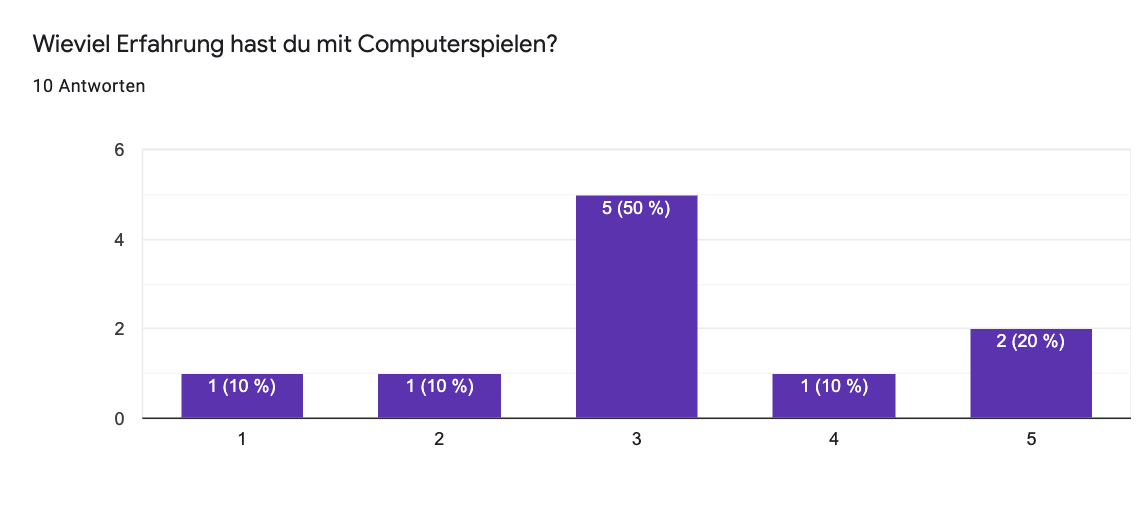
\includegraphics[width=0.99\textwidth]{images/erfahrungpc.png}
            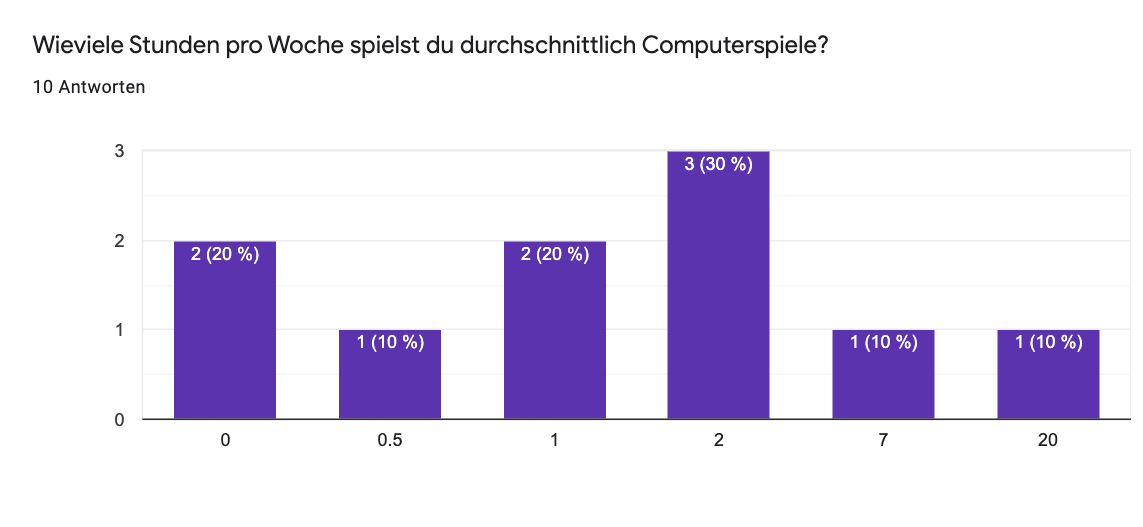
\includegraphics[width=0.99\textwidth]{images/pcstundenprowoche.png}
            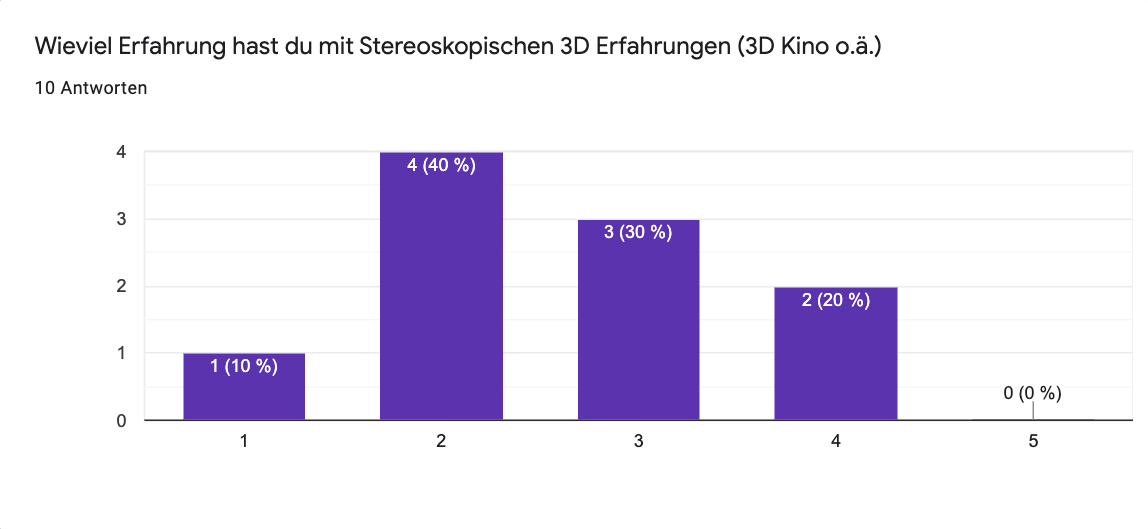
\includegraphics[width=0.99\textwidth]{images/3derfahrung.png}
            \caption{Angaben der Teilnehmenden zur Erfahrung mit Computerspielen und Stereoskopischem 3D.
            X-Achsen: Antworten der Teilnehmenden
            Y-Achsen: Häufigkeit der Antworten}\label{figure:videogames}
        \end{figure}

    \section{Ablauf der Studie}
        An dieser Stelle werde ich den genauen Ablauf der Studie beschreiben.
        Die Studie wurde zwischen dem 12.08.2021 und dem 20.08.2021 in einer geräumigen Wohnung in Hamburg/Stellingen ausgeführt. Nach Ankunft der Teilnehmer:innen wurden zunächst die notwendigen Covid-Sicherheitsmaßnahmen thematisiert.
        Zunächst haben diese sich ihre Hände desinfiziert, danach führten sie einen Antigen-Schnelltest an sich aus. In der Zeit, bevor das Ergebnis davon festgestellt werden konnten wurden den Proband:innen die Steuerung von der Joystick- und Teleportationsbedingung erklärt.
        Zudem wurde ihnen erklärt, dass ihre Aufgabe während des Experiments darin bestünde die fortbewegte Entfernung in jeder Bedingung einzuschätzen. Zudem sollen sie von Raum zu Raum gelanden indem sie an der Tür zum nächsten Raum die erforderlichen Zahlencodes eingeben, bis die Tür sich öffne. %formulierung

        Nachdem dann das negative Testergebnis abzulesen war (bei keiner Teilnehmer:in gab es ein positives Testergebnis), wurden die Proband:innen einer der Gruppen zugeteilt %wie?
        und ihnen wurde der in %link zum anhang mit demographie fragebogen
        abgebildete Demographie Fragebogen auf einem Laptop bereit gestellt. Nachdem dieser ausgeführt war durften die Proband:innen das erste mal die für die Durchführung der Studie genutzte Oculus Quest 2 Datenbrille aufsetzen um sich kurz damit vertraut zu machen. Nebenbei wurde das Bild der Brille über einen Google-Chromecast angezeigt, sodass es mir %?
        möglich war zu sehen, was in dieser dargestellt wurde. Den Teilnehmer:innen wurde erklärt wie sie innerhalb des Oculus Startbildschirm navigieren können, sodass diese dann selber die APK für die Studie öffnen konnten.
        %figure des menüs screenshot
        Nachdem diese geöffnet wurde (und der Unity-Ladebildschirm) abgeklungen war befanden die Teilnehmer:innen sich im virtuellen Menü der Studie(siehe abbildung x). Im Menü der Studie war die Teleportier-Fortbewegungsart aktiviert, damit die Teilnehmer:innen unabhängig der Reihenfolge, in der sie später die drei Bedingungen durchliefen schon einmal mit dieser vertraut waren.
        Dort befand sich auch das bereits in %TODO: chooserpad erklären
        \textquote{Chooser-Pad}, mit dem die Teilnehmenden dann sowohl ausprobieren konnten, wie die späteren Nummerneingabefelder funktionieren, also auch die Studienbedingung auswählen konnten. Dafür musste zuerst die entsprechende Taste ($A1-C3$, jeh nach Bedingung wie in \autoref{sec:setup} definiert) und danach die Bestätigungstaste \# gedrückt werden, mit der die Bedingung dann augenblicklich gestartet wurde. Den Proband:innen wurde, abhängig von ihrer Gruppe, mitgeteilt welche Bedingung sie ausführen sollen, dann starteten sie diese und führten sie aus.
        Nach Beendigung der Versuchsbedingung wurde den Proband:innen dann auf dem Laptop der Fragebogen %link zum zweiten Fragebogen
        geöffnet, den diese dann ausfüllten. Bei diesem wurde zuerst nach der Schätzung, gefragt (siehe \autoref{subsec:measure-distance}) und dann mithilfe des SUS-Questionaire %TODO:?
        nach dem Präsenzgefühl (siehe\autoref{subsec:measure-presence}).%TODO: links

        Das Öffnen, dann das Durchführen der Bedingung und das nachfolgende Ausfüllen des Fragebogens %formulierung
        wurde dann für jede der drei Bedingungen in der entsprechenden Reihenfolge durchgeführt. Danach wurde von mir überprüft ob die Daten, die am Ende einer Bedingung an die Firebase-Datenbank versendet werden, angekommen sind um im Falle eines Fehlers gegebenenfalls einzelne Bedingungen zu wiederholen. Dies ist erfreulicherweise nicht notwendig gewesen.

        Zu guter letzt wurden die Proband:innen gebeten die letzten, noch fehlenden Daten in den Demographiefragebogen zu füllen.

        %länge erwähnen
        %aufklärung überaschung?
        %marvs probleme?

        \section{Statistische Evaluationsverfahren}
            Im folgenden werde ich die statistischen Verfahren vorstellen, mit  denen ich die, im vorherigen Kapitel aufgestellten, Hypothesen   überprüfen werde.

            \subsection{Errechnung Qualität der Distanzschätzung}
            % errechnung % differenz positiv, negativ ?, signifikante unterschiede? abgleich mit literatur zur
                Die Qualität von der Schätzung der Proband:innen wird über die absolute Different zwischen gemessener Strecke und geschätzer Strecke, also folgendermaßen, berechnet:
                $$ \mid D_g - D_m \mid $$
                Wobei $D_g$ für die geschätze Distanz und $D_m$ für die gemessene Distanz steht.

            \subsection{Signifikanztests zur Distanzschätzung}
                Um die Unterschiede der errechneten Differenzen zwischen geschätzten und gemessenen fortbewegten Distanzen zu vergleichen und auf ihre Signifikanz zu testen bietet sich eine Varianzanalyse an.
                Aufgrund des \textquote{Within-Subjects Design} wird eine einfaktorielle Varianzanalyse mit Messwiederholung durchgeführt. Obwohl die verwendete Versuchsplanung auch eine zweifaktorielle Varianzanalyse ermöglichen würde, bei der die zweite abhängige Variable %?
                die Anzahl der durchlaufenen Räume ist, ist es nicht Ziel dieses Versuchs zu messen inwieweit sich diese Variable auf die Ergebnisse auswirkt.

                Um die für eine solche Varianzanalyse vorrausgesetze Normalität der verschiedenen Faktorstufen %?
                zu garantieren sollte vorher ein Shapiro-Wilk Test an diesen durchgeführt werden. Dieser eignet sich besonders gut dafür, da er auch bei sehr kleinen Stichproben aussagekräftig ist.

            \subsection{Signifikanztest über Ergebnisse des Präsenz-Questionaire}
                Ob die Unterschiede der Ergebnisse des SUS-Präsenz-Questionaire signfikant sind wird ebenfalls über eine einfaktorielle Varianzanalyse mit Messwiederholung ermittelt. Dabei werden die \textquote{SUS-Scores} der Durchläufe verglichen. Der SUS-Score ermittelt sich über die Anzahl der Fragen die mit dem Wert $6$ oder $7$, also die beiden Werte, die am meisten erlebte Präsenz beschreiben beantwortet wurden. %formulierung

                Auch hier muss ein Shapiro-Wilk Test die Vorraussetzung der Normalität der Faktorstufen überprüfen.

        \section{Auswertung der Ergebnisse}
            Die Daten aus den Google-Forms Formularen und die gemessenen Daten aus der Firebase Datenbank wurden jeweils anonym hinterlegt. Die Datensätze lassen sich einander lediglich über eine Versuchspersonen-ID, die Bedingung, und die Raumlänge %TODO: klar was gemeint ist? umschreiben?
            zuordnen.
            Um die Ergebnisse der beiden Quellen in einer gemeinsame Tabelle zu vereinen habe ich die Antworten auf das Google-Form in einer \textquote{Google-Tabellen}-Tabelle gesammelt und dann die Messergebnisse aus der Datenbank dazugetragen. Die Zuordnung erfolgte über die Versuchspersonen-ID, die Fortbewegungsbedingung und die Raumlänge%TODO: klar was gemeint ist? umschreiben?
            , die sich in beiden Datenquellen finden ließen und in der Kombination eindeutig einander zuordbar sind.
            Mit der Formel %link?
            berechnete ich eine neue Spalte, für die Differenz. Das ganze habe ich dann als $.csv$ Datei exportiert und um die weitere Datenverarbeitung und statistische in R durchzuführen. Dafür habe ich die Version \textquote{stable 4.1.1} genutzt.

                \subsection{Statistische Auswertung zur Schätzung der fortbewegten Distanz}
                    Die Auswertung zur Schätzung der fortbewegten Distanz erfolgt in zwei Teilen. Zuerst wird die Schätzung relativ zur tatsächlichen Distanz mit einer multiplen Varianzanalyse auf die Einflussfaktoren der Fortbewegungsart und der Raumanzahl des Levels untersucht.

                    Der zweite Teil untersucht die  absolute Differenz zwischen Schätzung und Distanz mit einer einfaktoriellen Varianzanalyse auf den Einfluss der Fortbewegungsart.

                    %%part 1
                    Das durchschnittliche Verhältnis zwischen Schätzung und gemessender Distanz ist $0,649$ (also circa $65\%$) bei einer Standartabweichung von $0,352$.

                    Die Durchschnittswerte und Standartabweichungen des Verhältnisses bei den einzelnen Fortbewegungsarten und Raumanzahlen steht in \autoref{table:ratio_means}

                    \begin{table}[]
                        \renewcommand\arraystretch{1.2}
                        \centering
            \begin{tabular}{lcccc} \toprule
                Bedingung       & Raumzahl & n   & M       & SD      \\ \midrule
                Redirection     & 3        & $3$ & $0,813$ & $0,298$  \\
                Redirection     & 6        & $3$ & $0,415$ & $0,356$  \\
                Redirection     & 9        & $3$ & $0,546$ & $0,183$  \\
                Joystick        & 3        & $3$ & $0,775$ & $0,319$  \\
                Joystick        & 6        & $3$ & $1,16$  & $0,422$  \\
                Joystick        & 9        & $3$ & $0,37$  & $0,298$  \\
                Teleport        & 3        & $3$ & $0,458$ & $0,343$  \\
                Teleport        & 6        & $3$ & $0,464$ & $0,199$  \\
                Teleport        & 9        & $3$ & $0,836$ & $0,051$  \\ \bottomrule
            \end{tabular}
                        \caption{Durchschnitte und Standartabweichungen des Verhältnisses zwischen gemessener und geschätzer fortbewegter Distanz; Alle Abweichungen sind bei einem $\alpha = 5\%$ Niveau nicht signifikant}\label{table:ratio_means}
                    \end{table}

                    Diese Ergebnisse werden auch in Form eines Boxplots in \autoref{figure:ratio-boxplot} abgebildet.

                    \begin{figure}[!h]
                        \centering
                        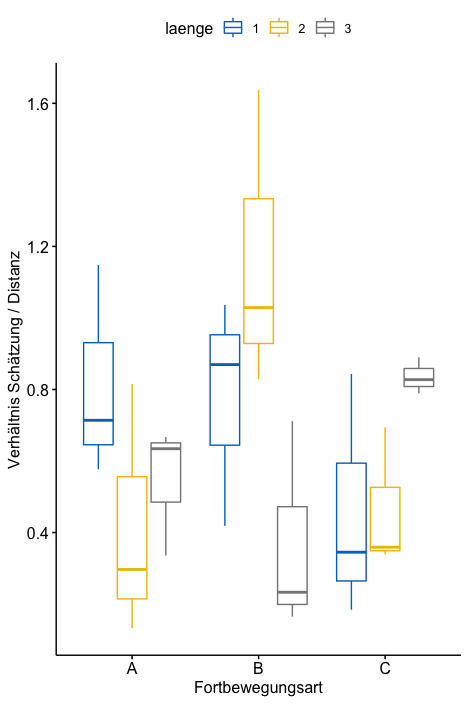
\includegraphics[width=1\textwidth]{plots/2wayboxplot.png}
                        \caption{Boxplot der Verhältnisse von geschätzer und gemessener fortbewegter Distanz; \textquote{laenge} meint die Raumanzahl der Level bei einer Kodierung von $1 = 3, 2 = 6$ und $3 = 9$ Räume pro Level}\label{figure:ratio-boxplot}
                    \end{figure}

                    Für eine zweifaktorielle Varianzanalyse müssen die einzelnen Faktorstufen der Daten normalverteilt sein.
                    Ein Plot der Korrelation zwischen den Faktorstufen (siehe \autoref{figure:qqplot-2way}) und ein Shapiro-Wilk-Test (siehe \autoref{table:shapiro-2way}) deuten nicht darauf hin, dass diese Bedingung verletzt wurde.

                    \begin{table}[]
                        \renewcommand\arraystretch{1.2}
                        \centering
        \begin{tabular}{lccc} \toprule
            Bedingung    & Raumanzahl & Teststatistik& $p$   \\ \midrule
            Real-Walking &  3         & $0,917$      & $0,442$ \\
            Real-Walking &  6         & $0,918$      & $0,445$ \\
            Real-Walking &  9         & $0,823$      & $0,172$ \\
            Joystick     &  3         & $0,934$      & $0,504$ \\
            Joystick     &  6         & $0,922$      & $0,459$ \\
            Joystick     &  9         & $0,842$      & $0,219$ \\
            Teleport     &  3         & $0,920$      & $0,451$ \\
            Teleport     &  6         & $0,792$      & $0,0959$ \\
            Teleport     &  9         & $0,981$      & $0,738$ \\ \bottomrule
        \end{tabular}
                        \caption{Die Ergebnisse eines Shapiro-Wilk Test der Werte für das Verhältnis zwischen Schätzung und Messung für die unterschiedlichen Fortbewegungsarten und Raumanzahlen; Die Annahme der Normalverteilung scheint bei einem Signifikanzniveau von $\alpha = 5\% $ für keine Faktorstufe verletzt}\label{table:shapiro-2way}
                    \end{table}

                    \begin{figure}[!h]
                        \centering
                        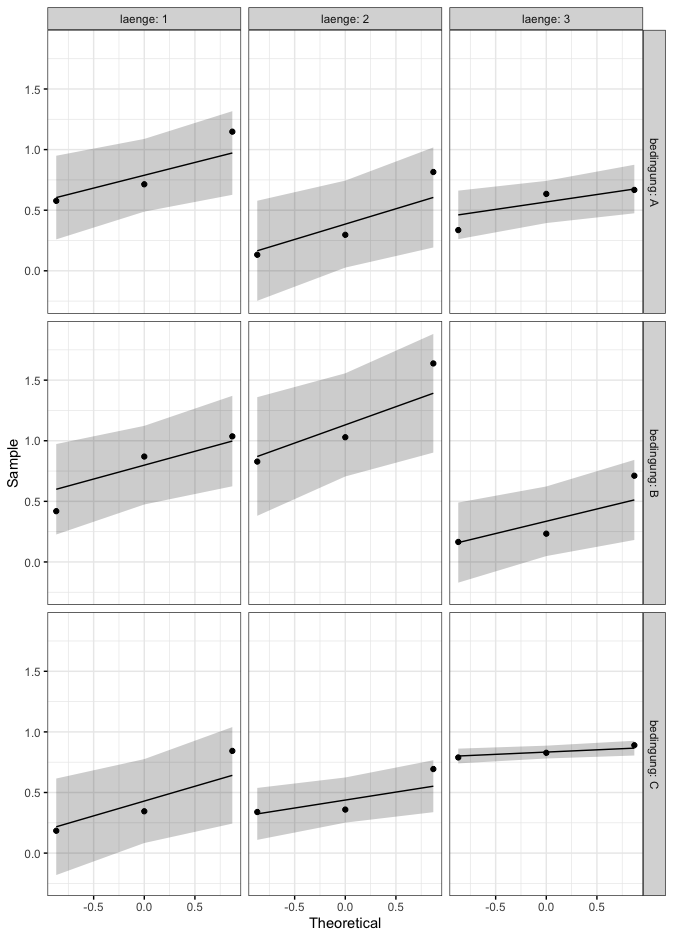
\includegraphics[width=1\textwidth]{plots/qqplot2way.png}
                        \caption{Plot der Korrelation zwischen den jeweiligen Faktorstufen und einer Normalverteilung; Mit laenge ist die Raumanzahl der Level mit einer Kodierung von $1 = 3, 2 = 6$ und $3 = 9$ gemeint}\label{figure:qqplot-2way}
                    \end{figure}


                    %%part 2

                    Durchschnittswerte der absoluten Differenz von Messung und Schätzung der fortbewegten Distanz sind in \autoref{table:diff_means} abgebildet.

                    \begin{table}[]
                        \renewcommand\arraystretch{1.2}
                        \centering
                        \begin{tabular}{lccc} \toprule
                            Bedingung       & n & M    & SD   \\ \midrule
                            Redirection     & $9$ & $16,9$ & $12,0$ \\
                            Joystick        & $9$ & $16,0$ & $16,8$ \\
                            Teleport        & $9$ & $13,8$ & $9,62$ \\ \bottomrule
                        \end{tabular}
                        \caption{Durchschnitte und Standartabweichungen der absoluten Differenz zwischen gemessener und geschätzer fortbewegter Distanz; Die Abweichungen sind bei einem $\alpha = 5\%$ Niveau nicht signifikant}\label{table:diff_means}
                    \end{table}

                    Ein Boxplot der Messergebnisse findet sich in \autoref{figure:diff_plot}

                    \begin{figure}[!h]
                        \centering
                        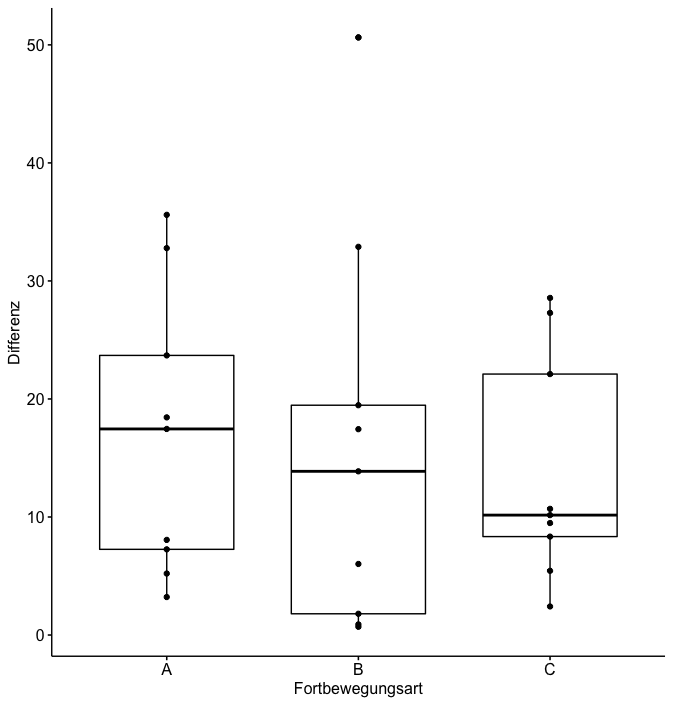
\includegraphics[width=1\textwidth]{plots/diff_plot.png}
                        \caption{Plot der Differenzen zwischen gemessener und geschätzer fortbewegter Distanz, Aufgeteilt nach Fortbewegungstechnik; A steht für Real-Walking, B für Joystick Steuerung und C für Teleportation}\label{figure:diff_plot}
                    \end{figure}

                    Eine Varianzanalye mit Messwiederholung setzt vorraus, dass die einzelnen Stufen des \textquote{Within-Subject Factor}, in diesem Fall die Fortbewegungsart, normalverteilt sind. Diese sind in \autoref{figure:diff_normality} abgebildet.

                    \begin{figure}[!h]
                        \centering
                        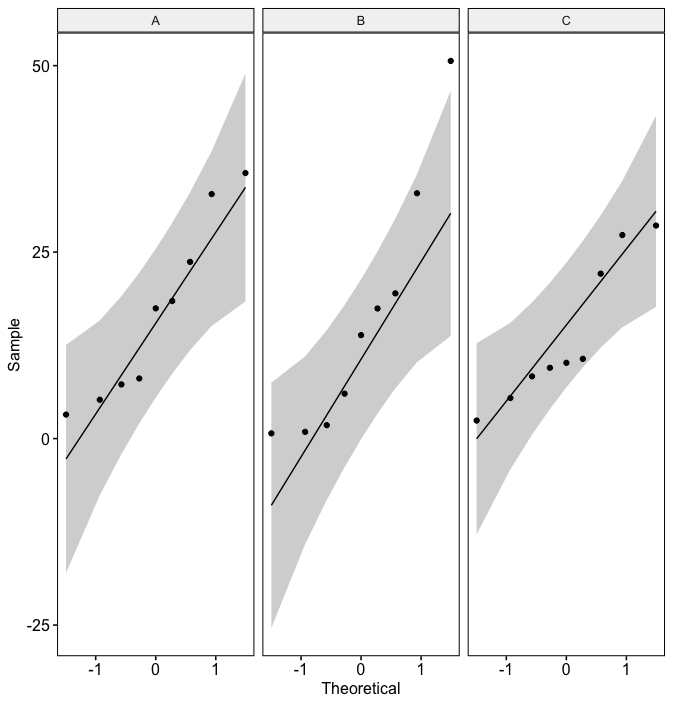
\includegraphics[width=0.5\textwidth]{plots/diff_normality.png}
                        \caption{Korrelation zwischen Messergebnissen und Normalverteilung nach Fortbewegungsart getrennt; A steht für Real-Walking, B für Joystick Steuerung und C für Teleportation}\label{figure:diff_normality}
                    \end{figure}

                    Zudem wurde ein Shapiro-Wilk Test für die einzelnen Faktorstufen durchgeführt (Ergebnisse in \autoref{table:norm_test_diff}). Dieser deutete nicht darauf hin, dass die Annahme der Normalverteilung verletzt worden sei.

                    %shapiro wilk diff
                    \begin{table}[]
                        \renewcommand\arraystretch{1.2}
                        \centering
                        \begin{tabular}{lcc} \toprule
                            Bedingung    & Teststatistik    & $p$   \\ \midrule
                            Real-Walking & $0,908$            & $0,300$ \\
                            Joystick     & $0,868$            & $0,117$ \\
                            Teleport     & $0,867$            & $0,113$ \\ \bottomrule
                        \end{tabular}
                        \caption{Die Ergebnisse eines Shapiro-Wilk Test der Werte für die Differenz von Schätzung und Messung für die unterschiedlichen Fortbewegungsarten; Die Annahme der Normalverteilung scheint für keine Faktorstufe verletzt; A steht für Real-Walking, B für Joystick Steuerung und C für Teleportation}\label{table:norm_test_diff}
                    \end{table}

                    Im Datensatz wurden keine extremen Ausreißer %grenze?
                    festgestellt.

                    Mit den erhobenen Daten wurde eine Varianzanalyse mit Messwiederholung zur Feststellung signifikanter Unterschiede zwischen den Fortbewegungsarten zum $\alpha = 5\%$ Level durchgeführt. Dabei wurde implizit ein Mauchly’s Test zur Überprüfung der Varianzhomogenität %das gleiche  wie spherecity? formulierung
                    durchgeführt. %TODO: Ergebnis davon beschreiben:
                    %mauchlys test for spherecity and greenhouse geisser correction

            %        When Mauchly’s test of sphericity indicated that the assumption of sphericity had been violated we used Greenhouse-Geisser estimates of sphericity to correct the degrees of freedom.

                    % $`Mauchly's Test for Sphericity`
                    % Effect     W     p p<.05
                    % 1 bedingung 0.457 0.064

% $`Sphericity Corrections`
%    Effect   GGe     DF[GG] p[GG] p[GG]<.05   HFe      DF[HF] p[HF] p[HF]<.05
% 1 bedingung 0.648 1.3, 10.37  0.72           0.721 1.44, 11.53 0.744

                    Die Varianzanalyse zeigte keine signifikanten Unterschiede zwischen den Fortbewegungsarten; $F(2,16) = 0.207, p = 0.815$
                    %anova diff
                    % 5% alpha, not significant F(2,16) = 0.207 p=0.815 ges = 0.01

                    Post-Hoc Tests zur genaueren Bestimmung der Unterschiede waren folglich nicht erforderlich.
%full:
%
    % > diff_aov
    % ANOVA Table (type III tests)

    % $ANOVA
    %      Effect DFn DFd     F     p p<.05  ges
    % 1 bedingung   2  16 0.207 0.815       0.01

    % $`Mauchly's Test for Sphericity`
    % Effect     W     p p<.05
    % 1 bedingung 0.457 0.064

    % $`Sphericity Corrections`
    %      Effect   GGe     DF[GG] p[GG] p[GG]<.05   HFe      DF[HF] p[HF] p[HF]<.05
    % 1 bedingung 0.648 1.3, 10.37  0.72           0.721 1.44, 11.53 0.744

%

%%%%%%%%%%%%%%%%%%%%%%%%%%%%%%%%%%%presence
                \subsection{Statistische Auswertung der Präsenz}
                    Für jeden Versuchsdurchlauf wurde der SUS-Score berechnet. Die Durchschnittswerte für die einzelnen Fortbewegungsarten sind in \autoref{table:presence_means} ersichtlich.

                    \begin{table}[]
                        \renewcommand\arraystretch{1.2}
                        \centering
                        \begin{tabular}{lccc} \toprule
                            Bedingung       & n & M     & SD   \\ \midrule
                            Real-Walking    & 9 & 2.33  & 1.80 \\
                            Joystick        & 9 & 0.889 & 1.36 \\
                            Teleport        & 9 & 0.667 & 0.866 \\ \bottomrule
                        \end{tabular}
                        \caption{Durchschnittswerte und Standartabweichungen der SUS-Scores für die verschiedenen Fortbewegungsarten; Die Unterschiede sind signfikant, können aber nicht von Post-Hoc Tests eingeordnet werden, denn dort sind die Ergebnisse nicht signifikant. %?????
                        } \label{table:presence_means}
                    \end{table}

                    \autoref{figure:presence_plot} Stellt die SUS-Scores als Boxplot dar. %wirklich? irgendwie komisch

                    \begin{figure}[!h]
                        \centering
                        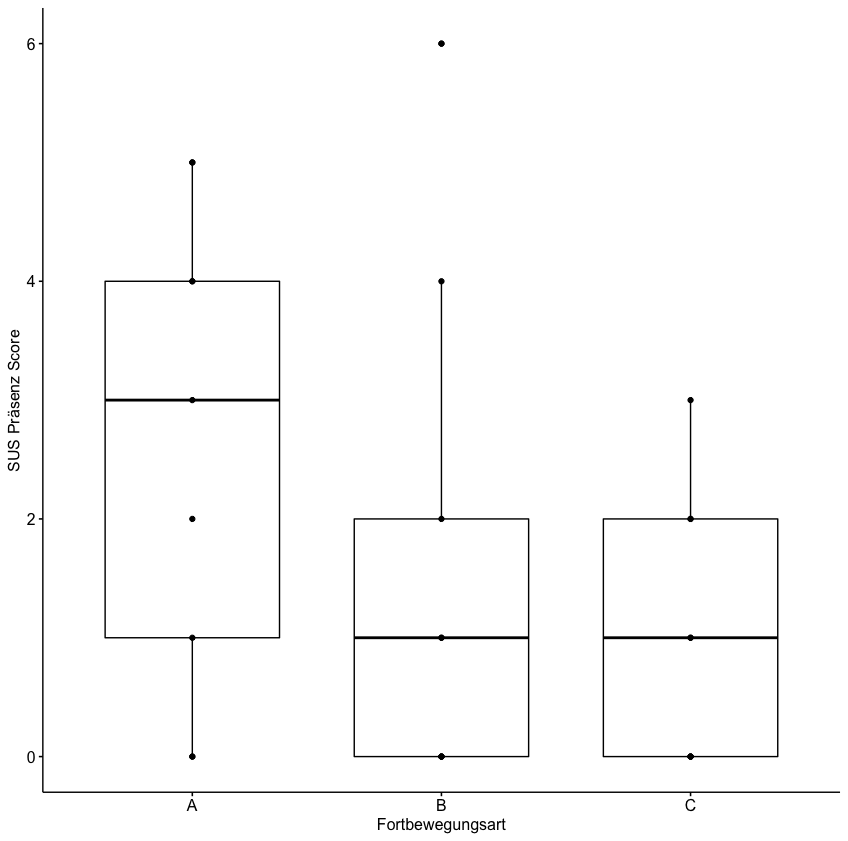
\includegraphics[width=1\textwidth]{plots/presence_plot.png}
                        \caption{Darstellung der SUS-Scores nach Fortbewegungsart;  A steht für Real-Walking, B für Joystick Steuerung und C für Teleportation}\label{figure:presence_plot}
                    \end{figure}

                    %no extreme outliers
                    Auch für die Präsenz-Messdaten wurden keine Extremen Ausreißer gefunden.

                    %qqplot
                    Die \autoref{figure:presence_normality} stellt die Korrelation zwischen den Daten und einer Normal-Verteilung für jede der Fortbewegungsarten dar.
                    Die Messpunkte in den Kategorien \textquote{Joystick} und \textquote{Teleportation} folgen nicht der Referenzlinie.

                    \begin{figure}[!h]
                        \centering
                        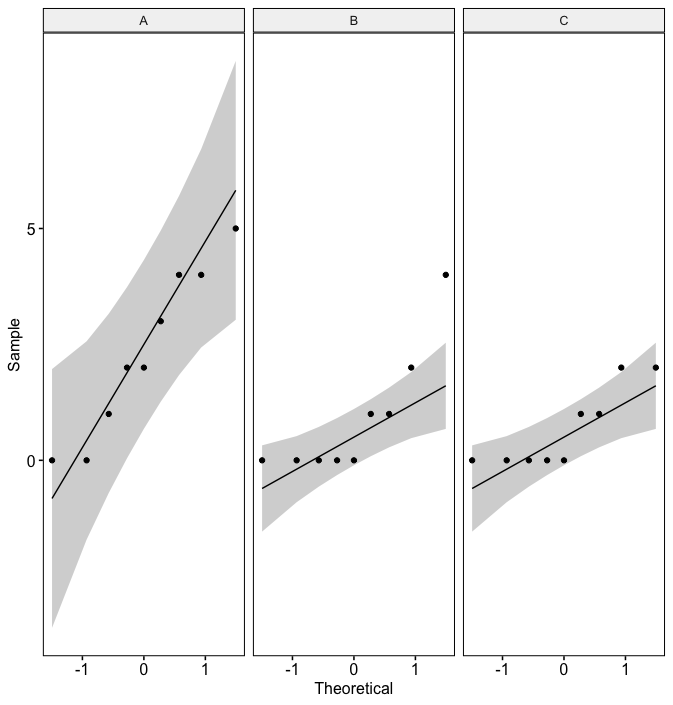
\includegraphics[width=0.5\textwidth]{plots/presence_normality.png}
                        \caption{Korrelation von SUS-Scores und Normalverteilung, nach Fortbewegungsart getrennt;  A steht für Real-Walking, B für Joystick Steuerung und C für Teleportation }\label{figure:presence_normality}
                    \end{figure}

                    Um Klarheit zu schaffen wurde ein Shapiro-Wilk test zum 5\% Konfidenzniveau %?
                    durchgeführt. Dieser weist darauf hin, dass eine Normalverteilung bei Joystick ($p = 0.00316$) und Teleportation ($p = 0.00521$) nicht gegeben ist. Die Ergebnisse des Shapiro-Wilk Tests sind in \autoref{table:presence_normal} zu sehen.

                    %shapiro
                    \begin{table}[!h]
                        \renewcommand\arraystretch{1.2}
                        \centering
                        \begin{tabular}{lccc} \toprule
                            Bedingung    & Teststatistik    & $p$   \\ \midrule
                            Real-Walking & 0.935            & 0.529 \\
                            Joystick     & 0.730            & 0.00316 \\
                            Teleport     & 0.748            & 0.00521 \\ \bottomrule
                        \end{tabular}
                        \caption{Ergebnisse eines Shapiro-Wilk Tests der verschiedenen Faktorstufen; Die Ergebnisse für die Joystick und die Teleportationsbedingung deuten bei einem $\alpha = 5\%$ Signifikanzniveau darauf hin, dass eine Normalverteilung nicht gegeben ist}\label{table:presence_normal}
                    \end{table}

                    Da die Bedingungen einer Varianzanalyse für die Daten zur Präsenzerhebung nicht eingehalten werden können wurde stattdessen ein Friedmann Test zur Feststellung signifikanter Unterschiede zwischen den Fortbewegungsarten zum $\alpha = 5\%$ Niveau durchgeführt.
                    %H0 erwähnen?
                    Dieser zeigte signifikante Unterschiede zwischen den Fortbewegungsarten; $\chi^2(2) = 9.3, p = 0.00956$

                    %friedman
                    %.y.           n statistic    df       p method
                    %* <chr>     <int>     <dbl> <dbl>   <dbl> <chr>
                    %1 sus_score     9       9.3     2 0.00956 Friedman test
                    Die Effektstärke wurde mithilfe einer  Kendall’schen Konkordanzanalyse errechnet. Dabei ergab sich eine Effektstärke von 0.517, dies gilt nach J.Cohen %source? TODO: %Cohen, J. (1988). Statistical Power Analysis for the Behavioral Sciences. Hoboken: Taylor and Francis.
                    als starker Effekt.

                    %effsize
                    %.y.           n effsize method    magnitude
                    %* <chr>     <int>   <dbl> <chr>     <ord>
                    %1 sus_score     9   0.517 Kendall W large

                    Dennoch wurden bei einer paarweise durchgeführten Post-Hoc Analyse der Präsenzdaten mit einem
                    Wilcoxon-Vorzeichen-Rang-Test mit Bonferroni-Korrektur der $p$-Werte keine signifikanten Unterschiede zwischen den jeweiligen Paaren von Fortbewegungsarten festgestellt. (Real-Walking mit Joystick: $p = 0.174$, Real-Walking mit Teleport: $p = 0.105$, Joystick mit Teleport: $p = 1$) Die Ergebnisse sind in \autoref{table:post-hoc-presence} dargestellt.

\begin{table}[!ht]
    \renewcommand\arraystretch{1.2}
    \centering
    \begin{tabular}{lcccc} \toprule
Gruppe 1     & Gruppe 2 & Teststatistik &  $p$  & $p$ korrigiert \\ \midrule
Real-Walking & Joystick & 15            & 0.058 & 0.174        \\
Real-Walking & Teleport & 21            & 0.035 & 0.105        \\
Joystick     & Teleport & 4.5           & 0.586 & 1     \\ \bottomrule
    \end{tabular}
    \caption{Ergebnisse der Post-Hoc Analyse mit Wilcoxon-Vorzeichen-Rang-Test; Die korrigierten $p$-Werte sind mithilfe der Bonferroni Korrektur korrigiert}\label{table:post-hoc-presence}
\end{table}

%post-hoc
% .y.       group1 group2    n1    n2 statistic     p p.adj p.adj.signif
% * <chr>     <chr>  <chr>  <int> <int>     <dbl> <dbl> <dbl> <chr>
% 1 sus_score A      B          9     9      15   0.058 0.174 ns
% 2 sus_score A      C          9     9      21   0.035 0.105 ns
% 3 sus_score B      C          9     9       4.5 0.586 1     ns


\chapter{Diskussion, Ausblick und Konklusion}\label{chapter:discussion-conclusion}
    In diesem letzten Kapitel werde ich die im vorherigen Kapitel errechneten Ergebnisse diskutieren und versuchen sie einzuordnen. Anschließend werde ich eine abschließende Zusammenfassung der in dieser Arbeit vorgestellten Ideen, Umsetzungen und Erkenntnissen geben. Damit verbunden werde ich einen Ausblick formulieren, wie zukünftige Forschungsarbeiten auf dieser Arbeit aufbauen sollten.

    \section{Diskussion der Ergebnisse}
        Die Ergebnisse liefern leider keine Unterstützung der vorgestellten Hypothesen. Dies könnte verschiedene Gründe haben. An dieser Stelle möchte ich versuchen die Ergebnisse einzuordnen und eben diese Gründe herauszuarbeiten

        \subsection{Schätzung der bewegten Distanz}
            Die oben formulierte Hypothese zur Schätzung der fortbewegten Distanz lautete wie folgt:

            Die \textquote{Real-Walking} Fortbewegungsart vereinfacht die Schätzung der fortbewegten Distanz im Vergleich zu den beiden alternativen \textquote{Joystick} und \textquote{Teleportation}.

            Die, in der hier vorgestellten Pilotierungsstudie, erhobenen Daten konnten diese Hypothese leider nicht stützen, die Gegenhypothese konnte nicht verworfen werden. Die Differenz der Fortbewegungsart \textquote{Real-Walking} ist nicht geringer, als die der Alternativen. Die Durchschnittswerte der unterschiedlichen Fortbewegungsbedingungen unterscheiden sich nicht signifikant. Ich möchte versuchen dafür einige mögliche Gründe herauszuarbeiten.

            Ein möglicher Grund dafür wieso diese Hypothese nicht unterstützt wird könnte sein, dass die vorher getroffene Annahme, die Schätzung der fortbewegten Distanz nähme mit besserem Raumverständnis zu, nicht zutrifft. %spricht da schon was für oder gegen?
            Zwar weist eine Post-Hoc Untersuchung von Peck et al. \cite{peck-vergleich-2011} darauf hin, dass Versuchspersonen bei einer Real-Walking Fortbewegungsbedingung, die Größe der virtuellen Umgebung besser einschätzen können, als bei alternativen virtuellen Fortbewegungsarten, allerdings bedeutet dies auch nicht zwingend, dass die Versuchspersonen ihre fortbewegte Distanz über mehrere Räume hinweg besser einschätzen können.

            In diesem Fall gäbe es mit der Real-Walking Fortbewegungsart zwar ein besseres Raumverständnis der Nutzer:innen, allerdings wäre diese von der hier angewandten Methode unentdeckt geblieben, da sie keine Auswirkungen darauf hätte, wie gut die Schätzungen sind.

            Alternative Möglichkeiten das Raumverständnis zu Messen sind beispielsweise, die Nutzer:innen zu bitten nach dem Durchschreiten des Levels eine Karte von diesem zu zeichnen, und die Genauigkeit der Karte dann von einer Jury bewerten zu lassen, oder wärend des Levels Objekte zu platzieren, auf die, die Proband:innen später zeigen müssen, und dann die Differenz der gezeigten Winkel mit den wahren winkeln zu vergleichen. (siehe \cite{peck-vergleich-2011, langbehn-vergleich-2018}).

            Ein möglicher weiterer Grund dafür wieso diese Hypothese nicht unterstützt werden konnte ist die Monotonität der generierten Räume.
            Die Räume unterscheiden sich voneinander nur unwesentlich, nämlich in Form der Seite des Raumes, an die der Korridor zum nächsten Raum generiert wird. Es liegt nahe, dass Nutzer:innen eine bessere kognitive Karte der Umgebung erzeugen könnten, wenn sie gewisse Anhaltspunkte hätten, an die sie sich erinnern könnten. Dies lässt sich begrenzt verbessern, indem bei der Levelgenerierung in die Räume vordefinierte Objekte platziert werden. Dennoch ist eben dies ein Grundproblem von generierten (generischen) Leveln.

            Falls die oben erwähnte Annahme doch zutrifft, könnte es also sein, dass sich die Fähigkeit von Nutzer:innen, die fortbewegte Distanz einzuschätzen, zwischen von Menschen gestalteten und Computergenerierten Leveln signifikant unterscheidet.

            Dies, und ob das Raumverständnis einer Person, mit der Fähigkeit fortbewegte Distanz einzuschätzen in kausalem Zusammenhang steht sollte in einer zukünftigen Studie untersucht werden. Dafür könnten die eben beschriebenen Möglichkeiten das Raumverständnis zu messen genutzt werden. Es wäre dann sinnvoll die Level nach ihrer Generierung zu Speichern und zu exportieren, sodass die Beschreibungen der Proband:innen mit den wirklich generierten Leveln verglichen werden können. Ausserdem sollten die Level um zufällig in die Räume platzierte Objekte und anderen Varianzen zwischen den Räumen ersetzt werden, da dies die kognitive Kartenbildung mutmaßlich vereinfacht.
            %weitere gründe?

        \subsection{Präsenzgefühl in der virtuellen Umgebung}
            Die oben formulierte Hypothese zum Präsenzgefühl lautete:

            Mit der \textquote{Real-Walking} Fortbewegungsart haben Nutzer:innen ein größeres Präsenzgefühl als mit den beiden alternativen \textquote{Joystick} und \textquote{Teleportation}.

            Der Durchschnittswert der SUS-Präsenz-Scores ist bei der Real-Walking Testbedingung ($2.33$) ist deutlich größer, als bei der Joystick-($0.889$) oder Teleportationsbedingung ($0.667$).
            Leider kann für diese Hypothese in den hier erhobenen Daten dennoch keine Unterstützung gefunden werden. Zwar weist ein statistischer Test der Präsenz-Scores der drei Fortbewegungsarten auf signifikante Unterschiede, sogar mit starker Effektstärke hin, allerdings lassen sich in den darauf folgenden Tests, in denen die 3 Fortbewegungsarten paarweise miteinander verglichen werden keine signifikanten Unterschiede feststellen.

            Ein möglicher Grund für diese ambivalenten Ergebnisse hat konkret mit den Umständen %link?
            dieser Studie zu tun. Da nicht so viele Proband:innen teilnehmen konnten, wie es üblicherweise der Fall gewesen wäre, ist die Datenlage, aus der diese Ergebnisse entstanden weniger gut, als sie in einer offiziellen Studie gewesen wäre. %formuliereung
            Es ist davon auszugehen, dass die Ergebnisse in diesem Fall um einiges klarer gewesen wären.

            Folglich ist es wünschenswert diese Frage in einem größerem Kontext genauer zu untersuchen. %?

    \section{Konklusion}
        In dieser Arbeit wurde eine Methode zur prozeduralen Generierung von Raum-Basierten Leveln für virtuelle Umgebungen vorgestellt, bei der  Nutzer:innen, mithilfe von Rotationgains und Impossible Spaces, ermöglicht wird sich mit natürlichem Gehen auf eine Weise von Raum zu Raum fortzubewegen, bei der die Illusion entsteht sie würden die Grenzen des realen Trackingspaces verlassen und könnten unabhängig davon die virtuelle Umgebung erkunden. Diese Methodik ermöglicht potentiell unendlich lange Level, bei denen die Generierung während der Erkundung des Levels fortgeführt wird.

        Anschließend wurde eine informelle Pilotierungsstudie vorgestellt und durchgeführt, bei der drei verschiedene Fortbewegungsarten in, mit dieser Methode generierten, Leveln verglichen wurden. Dabei wurde versucht zwei Vorteile, die die Ermöglichung echten Gehens in virtuellen Umgebungen bieten könnte, nämlich eine vereinfachte Schätzung fortbewegter Distanzen und ein erhöhtes Präsenzgefühl für Nutzer:innen, zu zeigen. Dies könnte sowohl an der, den Umständen geschuldeten geringen Datenlage von 10 Versuchspersonen liegen, als auch daran, dass diese Vorteile nicht in prozedural generierten Leveln gegeben sind. %autsch

    \section{Ausblick}

        Wie bereits erwähnt sind die Ergebnisse der hier durchgeführten Pilotierungsstudie mit einer relativ geringen Teilnehmerzahl entstanden. Um die Ergebnisse mit mehr Genauigkeit beurteilen zu können wäre es wünschenswert wenn eine etwas größere,  offizielle Studie mit den hier vorgestellten Methoden durchgeführt würde.
        Aber auch abgesehen davon gibt es einige Fragen, die in dem Prozess dieser Arbeit aufgeworfen wurden, deren Klärung es bedarf.

        Zukünftige Studien, die Level mit der hier vorgestellten Methode generieren sollten untersuchen, inwieweit eine Generierung von Objekten in den Räumen zur kognitiven Kartenbildung von Nutzer:innen beiträgt. Außerdem sollte sie, anstatt nur die Qualität der Distanzschätzung zu untersuchen auch Forschungsmethodiken nutzen, die auf andere Art und Weisen das Raumverständnis der Proband:innen prüfen.
        %noch mehr finden?


\chapter*{Danksagungen}\label{chapter:acknowledgements}
\addcontentsline{toc}{chapter}{Danksagungen}
    An dieser Stelle möchte ich mich bei allen bedanken, die mich während diesem Projekt unterstützt und motiviert haben.
    Ganz herzlicher Dank gebürt bei all meinen Freunden und Verwandten, die freundlicherweise an der Studie teilgenommen haben! Ganz besonderer Dank geht dabei an meine Eltern, Jutta Dalladas-Djemai und Chaffok Djemai, für die vielen Jahre Unterstützung, die mir ermöglicht haben zu Studieren und abzuschließen, und an meine Freundin Nora Schwerdtfeger, die mich in schwierigen Phasen stets motiviert hat.
    Außerdem möchte ich mich bei meinem Betreuer Dr. Eike Langbehn bedanken, dessen Expertise und Gedult mir die Arbeit an diesem Projekt erleichtert hat.

%%%%%%%%%%%%%%%%%%%%%%%%%%%%%%%%%%%%%%%%%%%%%%%%%%
    %TODO: auf peck verweisen ===>
        %Moreover, RFED participants were able to more accurately estimate VE size.

% keep an blank line above